\documentclass[12pt,twoside,a4paper,bibliography=totocnumbered]{book}



\usepackage[utf8]{inputenc}
\usepackage[T1]{fontenc}
\usepackage{lmodern}
\usepackage{amsmath,amssymb,amsthm}
\usepackage{mathabx}\changenotsign
\usepackage{mathrsfs}
\usepackage{dsfont}
\usepackage[babel]{microtype}
\usepackage{xcolor}  	
\usepackage[backref]{hyperref}
\usepackage{mathtools}
\usepackage{indentfirst}
\usepackage{graphicx} % Gerencia imagens incluidas
\usepackage{float} 
\usepackage{bbm}

\hypersetup{
	colorlinks,
    linkcolor={red!60!black},
    citecolor={green!60!black},
    urlcolor={blue!60!black},
}

%\usepackage{bookmark}

\usepackage[abbrev,msc-links,backrefs]{amsrefs}
\usepackage{doi}
\renewcommand{\doitext}{DOI\,}

\renewcommand{\PrintDOI}[1]{\doi{#1}}

\renewcommand{\eprint}[1]{\href{http://arxiv.org/abs/#1}{arXiv:#1}}


\usepackage[T1]{fontenc}
\usepackage{lmodern}

\usepackage[english]{babel}
\numberwithin{equation}{section}

\linespread{1.3}
\usepackage{amsfonts}
\usepackage{geometry}
\geometry{left=27.5mm,right=27.5mm, top=25mm, bottom=25mm}


\usepackage{enumitem}
\def\rmlabel{\upshape({\itshape \roman*\,})}
\def\RMlabel{\upshape(\Roman*)}
\def\alabel{\upshape({\itshape \alph*\,})}
\def\Alabel{\upshape({\itshape \Alph*\,})}
\def\nlabel{\upshape({\itshape \arabic*\,})}

\def\aplabel{\upshape({\itshape \alph*\,$'$})}

\let\polishlcross=\l
\def\l{\ifmmode\ell\else\polishlcross\fi}

\def\tand{\ \text{and}\ }
\def\qand{\quad\text{and}\quad}
\def\qqand{\qquad\text{and}\qquad}

\let\emptyset=\varnothing
\let\setminus=\smallsetminus
\let\backslash=\smallsetminus
%\let\subset\subseteq
\let\log=\ln

\newcommand\mc{\mathop{\textrm{\rm mc}}\nolimits}

\makeatletter
\def\moverlay{\mathpalette\mov@rlay}
\def\mov@rlay#1#2{\leavevmode\vtop{   \baselineskip\z@skip \lineskiplimit-\maxdimen
   \ialign{\hfil$\m@th#1##$\hfil\cr#2\crcr}}}
\newcommand{\charfusion}[3][\mathord]{
    #1{\ifx#1\mathop\vphantom{#2}\fi
        \mathpalette\mov@rlay{#2\cr#3}
      }
    \ifx#1\mathop\expandafter\displaylimits\fi}
\makeatother

\DeclareMathOperator{\dom}{{\rm dom}}

\newcommand{\dcup}{\charfusion[\mathbin]{\cup}{\cdot}}
\newcommand{\bigdcup}{\charfusion[\mathop]{\bigcup}{\cdot}}


\DeclareFontFamily{U}  {MnSymbolC}{}
\DeclareSymbolFont{MnSyC}         {U}  {MnSymbolC}{m}{n}
\DeclareFontShape{U}{MnSymbolC}{m}{n}{
    <-6>  MnSymbolC5
   <6-7>  MnSymbolC6
   <7-8>  MnSymbolC7
   <8-9>  MnSymbolC8
   <9-10> MnSymbolC9
  <10-12> MnSymbolC10
  <12->   MnSymbolC12}{}
\DeclareMathSymbol{\powerset}{\mathord}{MnSyC}{180}



\makeatletter
\def\namedlabel#1#2{\begingroup
    #2%
    \def\@currentlabel{#2}%
    \phantomsection\label{#1}\endgroup
}
\makeatother


\newtheorem{theorem}             {Theorem}[section]
\newtheorem{lemma}     	[theorem] {Lemma}
\newtheorem{conjecture}	[theorem] {Conjecture}
\newtheorem{property}  	[theorem] {Property}
\newtheorem{definition}	[theorem] {Definition}
\newtheorem{proposition}[theorem] {Proposition}
\newtheorem{corollary}	[theorem] {Corollary}
\newtheorem{fact}	[theorem] {Fact}
\newtheorem{claim}	[theorem] {Claim}

\newtheoremstyle{remark}  {2pt}  {4pt}  {\rm}  {}  {\bfseries}  {.}  {.3em}          {}
\theoremstyle{remark}
\newtheorem{remark}	[theorem] {Remark}
\newtheorem{example}	[theorem] {Example}

\renewcommand{\thefootnote}{\fnsymbol{footnote}}

\let\eps=\varepsilon
\let\theta=\vartheta
\let\rho=\varrho
\let\phi=\varphi


\def\NN{\mathds N}
\def\ZZ{\mathds Z}
\def\QQ{\mathds Q}
\def\RR{\mathds R}
\def\PP{\mathds P}
\def\EE{\mathds E}

\def\cB{\mathcal B}
\def\cR{\mathcal R}

\def\ra{\longrightarrow}
\usepackage{centernot}
\def\nra{\centernot\longrightarrow}
\def\red{\text{\rm red}}
\def\blue{\text{\rm blue}}
\def\green{\text{\rm green}}
\def\R{\text{\rm red}}
\def\B{\text{\rm blue}}

\def\ex{\mathop{\text{\rm ex}}\nolimits}





\usepackage{datetime}
\usepackage{lineno}
\newcommand*\patchAmsMathEnvironmentForLineno[1]{%
\expandafter\let\csname old#1\expandafter\endcsname\csname #1\endcsname
\expandafter\let\csname oldend#1\expandafter\endcsname\csname end#1\endcsname
\renewenvironment{#1}%
{\linenomath\csname old#1\endcsname}%
{\csname oldend#1\endcsname\endlinenomath}}%
\newcommand*\patchBothAmsMathEnvironmentsForLineno[1]{%
\patchAmsMathEnvironmentForLineno{#1}%
\patchAmsMathEnvironmentForLineno{#1*}}%
\AtBeginDocument{%
\patchBothAmsMathEnvironmentsForLineno{equation}%
\patchBothAmsMathEnvironmentsForLineno{align}%
\patchBothAmsMathEnvironmentsForLineno{flalign}%
\patchBothAmsMathEnvironmentsForLineno{alignat}%
\patchBothAmsMathEnvironmentsForLineno{gather}%
\patchBothAmsMathEnvironmentsForLineno{multline}%
}
\usepackage{graphicx}

\begin{document}
%\linenumbers

\title{Extremal and Probabilistic Combinatorics}

      \begin{figure}[h!]%
        \centering%
        
\includegraphics[scale=0.2]{Figuras/logo.png}%
      \end{figure}%     
\begin{center}
Universidade Federal do ABC\\

\vspace{2cm}

{
\fontsize{18pt}{\baselineskip}\selectfont \bf
Extremal and Probabilistic Combinatorics
}

\vspace{2cm}

Diogo Eduardo Lima Alves\\

\vspace{2cm}

UNDERGRADUATE PROJECT IN COMPUTER SCIENCE PRESENTED\\
TO\\
CENTER OF MATHEMATICS, COMPUTATION AND COGNITION\\
OF\\
FEDERAL UNIVERSITY OF ABC\\
FOR\\
OBTAINING TITLE\\
OF\\
COMPUTER SCIENCE BACHELOR\\
\vspace{2cm}
Advisor: Prof. Dr. Guilherme Oliveira Mota\\
\vfill
Santo André - SP\\
May 2019
\end{center}

\newpage
\begin{center}
Diogo Eduardo Lima Alves
\end{center}
   \begin{center}
        \vspace*{4 cm}
        \textbf{\Large{Extremal and Probabilistic Combinatorics}}\\
        \vspace*{5cm}
    \end{center}

    \begin{flushright}
{\bf Undergraduate Project} presented to\\ 
Undergraduate Program in Computer Science\\ 
(Concentration area: Graph Theory),\\ 
as partial requirement to obtain the title\\ 
of Bachelor in Computer Science.
    \end{flushright}

\vspace{3cm}
\begin{center}
Advisor: Prof. Dr. Guilherme Oliveira Mota\\
\vfill
Santo André - SP\\
May 2019
\end{center}

\tableofcontents

\listoffigures
%\listoftables

\chapter{Introduction}
Computer Science was truly fundamental for the fast development of science in the last century, also being fundamental to its validation and communication. It is really hard to think about actual science without the use of computers or strong science communities connected and accessible by the internet. Computer Science is also essential for business. All multinational companies are also software companies since the way of production, operating and delivering products are managed by softwares and these aspects are determinants for the success level of any company in the world. It is also common that one of the most valuable assets of a company can be connected to data, software and algorithms. In this scenario, graphs are also very interesting due its importance to Computer Science.

Graphs are one of the most flexible structures, impacting the study of Algebra, Probability and Combinatorics. They can be used for modeling many real scenarios in a very understandable graphical scheme and its properties can be explored to obtain many useful information what explains its huge importance for many knowledge areas not directly connected to Computer Science or Mathematics.   

This project focus on classical results of Extremal Combinatorics and Graph Theory. It has detailed ideas and explanations about theorems and concepts developed through a large period of time which have already been intensively studied.

Extremal Combinatorics studies the maximum or minimum size a collection of objects may have while satisfying certain restrictions. We are particulary interested on graphs and their substructures. 

Extremal Graph Theory studies graphs' possible sizes at the same time they hold some property, which can involve bounds on the number of edges and vertices, since this property, in general, is the absence of a specific subgraph.

Ramsey Theory, roughly speaking, is the study of finding order in chaos and studies the conditions under which order must appear.

The Probabilistic Method is a very useful tool, because it is flexible and it is used to prove the existence of a structure with certain properties. We define a probability space and pick randomly an element of this space then we show this element has the desired properties with positive probability.

Finally the regularity lemma is discussed, one of the most important tools in Combinatorics, informally it is about acquiring from any graph a good approximation with random-like subgraphs which gives us a huge flexibility to prove many statements.

%\chapter{Justification}
%ME INTERESSEI PELO TEMA, APENAS!


%\chapter{Objectives}



%\chapter{Methodology}
%The main bibliography referential material used in this project is the book ``Extremal and Probabilistic Combinatorics'' written by Robert Morris and Roberto Imbuzeiro Oliveira which is part of Impa's mathematical publications and is a result of a Extremal Combinatorics course.

%Almost all the doubts and problems about proofs, explanations and structure over the entire text construction was supported by the projects' advisor, the professor Dr. Guilherme Oliveira Mota.

\chapter{Preliminaries}
In this chapter we introduce concepts and state the basic notation to be used in the next chapters.

\section{Numbers and Sets}
We use $\mathbb{N} = \{1,2,...\}$ to denote the set of positive integers, and $[n]=\{1,...,n\}$ denotes the set of all positive integers from $1$ to $n$. 

For a set $S$, we use $|S|$ to denote the number of elements of $S$. We state $\binom{S}{k}$ as the set of all subsets of $S$ with size $k$ and use $\{x_1,...,x_k\}$ to detone an element in $\binom{S}{k}$. For $|S| = n$ and $0 \leq k \leq n$ the number of elements in $\binom{S}{k}$ is the binomial coefficient
$$ \left| \binom{S}{k} \right| = \binom{n}{k} = \frac{n!}{k!(n-k)!}.$$

For a graph $G$ an indenpendent set $I$ is a subgraph of $V(G)$, $I \subseteq V(G)$, such that for every $\{u\}$ and $\{v\}$ in $I$ the edge $\{u,v\}$ is not in $E(G)$.
 
\section{Asymptotics}
We write $f(n) = o(g(n))$ if and only if, for all $\varepsilon > 0$, there exist $n_0$ such that if $n \geq n_0$, then $f(n) < \varepsilon g(n)$. We can write sometimes $f(n) \ll g(n)$ instead of $f(n) = o(g(n))$.

We have $f(n) \approx g(n)$ if $f(n)/g(n) \rightarrow 1$ as $n \rightarrow \infty$.

\section{Graphs}
A graph $G = (V(G), E(G))$ or simply $G = (V, E)$ is a pair formed by the set of vertices $V(G) = [n]$, with $|V(G)|=n$ and the set of edges, $E(G) \subseteq \binom{V(G)}{2}$, is formed by pairs of vertices. We can represent an edge $e = \{u,v\}$ as simply $uv$ and a vertex $\{v\}$ as simply $v$. And we use $e(G) = |E(G)|$ and $v(G) = |V(G)|$.

A $s$-clique, $K_s = (V(K_s),E(K_s))$, is a pair formed by the set of vertices $V(K_s) =  [s]$ and the set of edges $E(K_s) = \binom{V(K_s)}{2}$.

A vertex colouring with $r$ colours in a graph $G$ is a function $c\colon V(G) \rightarrow \{1,...,r\}$ and it can also be denoted as a $r$-colouring of the vertices of $G$. We denote the colour $i$ of a vertex $v$ as $c(v)=i$. If we have a graph $Z$ such that $c(z)=i$ for every $z$ in $V(Z)$ we call it monochromatic or monochromatic in colour $i$.


An edge colouring with $r$ colours in a graph $G$ is a function $c\colon \binom{V(G)}{2} \rightarrow \{1,...,r\}$ and it can also be denoted as a $r$-colouring of the edges of $G$. We denote the colour $i$ of an edge $\{u,v\}$ as $c(\{u,v\})=i$. If we have a graph $W$ such that $c(\{u,v\})=i$ for every $\{u,v\}$ in $E(W)$ we call it monochromatic or monochromatic in colour $i$.

Let $G$ and $H$ be graphs such that $V(H) \subseteq V(G)$ and $V(G)= [n]$. We define $\ex(n,H) = \max\{e(G): E(H)\text{ is not in }E(G)\}$. If $H$ is not in $G$ we call $G$ a $H$-free graph.

\section{Adjacent and Incident}
Given an edge $e =\{u,v\}$ in a graph $G$ we call $u$ and $v$ neighbours or adjacents and we can denonte $e =\{u,v\}$ as $u$ is neighbour of $v$ or $u$ is adjacent to $v$. We also say the edge $\{u,v\}$ is incident to $u$ and $v$.

The degree of a vertex $v$ in a graph $G$, denoted by $d_G(v)$, we also write simply $d(v)$, is the quantity of neighbours of $v$. The set of neighbours of $v$ is called neighbourhood and is denoted by $N_G(v)$ or simply $N(v)$.

The minimum degree of a graph $G$ is denoted by $\delta(G)$ and is defined as
$$\delta(G) = \min\{d(v) \colon v \in V (G)\}.$$

The maximum degree of a graph $G$ is denoted by $\Delta(G)$ and is defined as 
$$ \Delta(G) = \max\{d(v) \colon v \in V(G)\} $$

\section{Probability}
In this text, we call by probability space a non-empty finite set $\Omega$ and we write a function $\mathbb{P}\colon \Omega \rightarrow [0,1]$ that relates a probability $\mathbb{P}(\omega)$ to each $\omega$ in $\Omega$. In any, case the probabilities are assumed to satisfy
$$ \sum_{\omega \in \Omega} \mathbb{P}(\omega) = 1.$$

Subsets $E \subseteq \Omega$ are called events, and we write $\mathbb{P}(E) = \sum_{\omega \in E}\mathbb{P}(\omega)$. The Inclusion-Exclusion principle shows that, for all $E_1, E_2 \subseteq \Omega$

$$ \mathbb{P}(E_1 \cup E_2) = \mathbb{P}(E_1) + \mathbb{P}(E_2) - \mathbb{P}(E_1 \cap E_2) \leq \mathbb{P}(E_1) + \mathbb{P}(E_2).$$

A mapping $X\colon \Omega \rightarrow \mathbb{R}$ is called a random variable and the expected value of $X$ is given by

$$ \mathbb{E}[X] = \sum_{\omega \in \Omega}X(\omega)\mathbb{P}(\omega) .$$

The variance of $X$ is Var$(X) = \mathbb{E}(X^2) - \mathbb{E}(X)^2$. We usually write $X > t$ and $X = x$ to denote the events $\{\omega 
\in \Omega \colon X(\omega) > t\}$ and $\{\omega \in \Omega \colon X(\omega) = x\}$, respectively. In the text we usually omit the probability space information and focus on events and ramdom variables. 

A sequence of events $E_1,...,E_m \subseteq \Omega$ is independent if for every $M \subseteq [m]$ and $M \neq \emptyset$,

$$ \mathbb{P}\left( \bigwedge_{i \in M}E_i \right) = \prod_{i \in M} \mathbb{P}(E_i).$$

\chapter{Ramsey Theory}

Ramsey's Theory is especially philosophical among the components of the Extremal Combinatorics. Ramsey's Theory is connected with the purpose of finding order in chaos, that is, it is motivated by the thought that complete chaos is impossible to achieve, then we can prove statements about any graph, independent of its particular characteristics.

\section{Infinite Ramsey's Theorem}
Consider the following question:
``Given a group of 6 people, are there 3 people that are mutual friends or 3 people that are mutual strangers?''

In order to answer this question think about a group of six people, call them Richard, Maria, Bete, Jack, Paul and Steven. It is possible to suppose without loss of generality that Richard has at least three friends: Maria, Bete and Jack. If any two of these three are friends with each other, then they form a group of three mutual friends with Richard, otherwise Maria, Bete and Jack form a group of three mutual strangers to themselves. 

Replacing people by vertices and a friendship by colours (blue for being friends and red otherwise) we realize that a graph $G$ with $6$ vertices always have a monochromatic triangle independently of the edge colouring, but what about with $5$ vertices?

The graph $K_5$ can be constructed without a monochromatic triangle as show in Figure \ref{fig:K5}. The following definition will permit us to discuss it in terms of the Ramsey Numbers.

\begin{definition}\label{def:RamseyNumbers} 
The Ramsey Number $R(s,t)$ is the minimum $n$ such that any $2$-colouring on $\binom{K_n}{2}$ induces a complete subgraph $K_s$ whose edges are monochromatic in colour $1$ or a complete subgraph $K_t$ whose edges are monochromatic in colour $2$.
\end{definition}

Then using the Definition \ref{def:RamseyNumbers} we have $R(3,3) = 6$.

\begin{figure}[H]
     \centering
     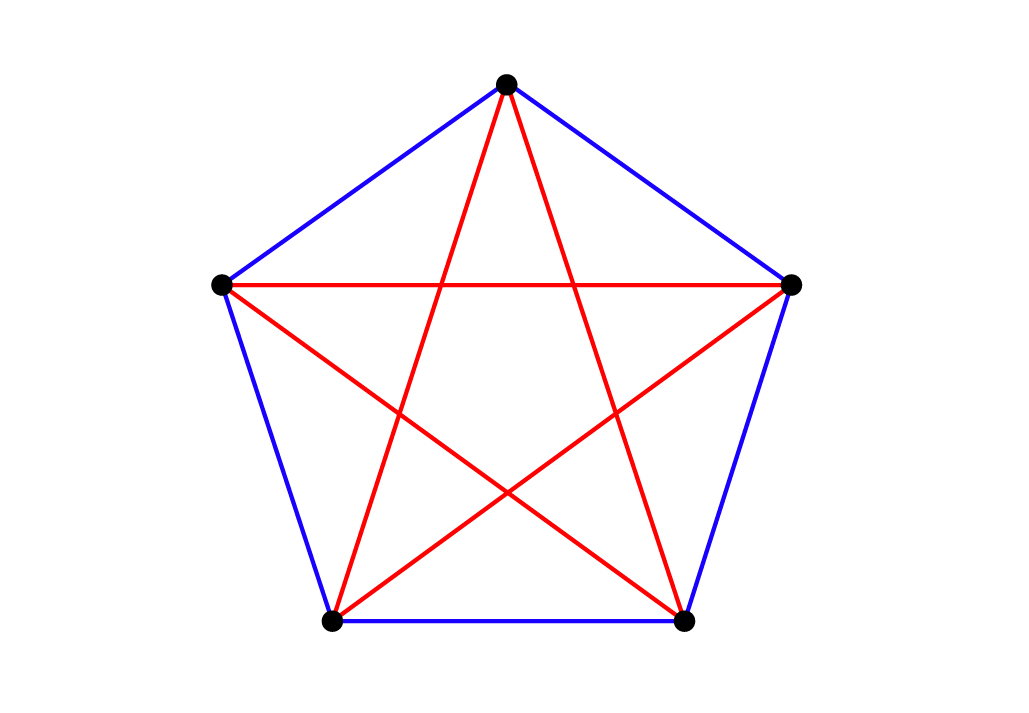
\includegraphics[scale=1]{Figuras/K5-sem-triangulo.jpg}
     \caption{Graph $K_5$ without monochromatic triangle.}
     \label{fig:K5}
\end{figure}

\begin{theorem}[{Ramsey's Theorem - Infinite Version \cite{Ra29}}]\label{thm:RamseyTheorem}
Let $r \geq 1$ be an integer. Every colouring $c\colon \dbinom{\mathbb{N}}{2}$ $\rightarrow$ $[r]$ implies an infinite monochromatic subset of $\mathbb{N}$.
\end{theorem}

Revisar.Revisar.Revisar.Revisar.Revisar.Revisar.Revisar.

Revisar.Revisar.Revisar.Revisar.Revisar.Revisar.Revisar.

Revisar.Revisar.Revisar.Revisar.Revisar.Revisar.Revisar.

Revisar.Revisar.Revisar.Revisar.Revisar.Revisar.

\section{Schur's Theorem}

\begin{theorem}[{Schur's Theorem \cite{Sc16}}]\label{thm:Schur'sTheorem} %Schur, 1916
For any positive integer and any colouring $c\colon \mathbb{N} \rightarrow [r]$, there are $a,b,c$ such that $a+b=c$ and $c(a) = c(b) = c(c)$.
\end{theorem}
\begin{proof}
  For a vertex colouring given as $c\colon \mathbb{N} \rightarrow [r]$ define an edge colouring $c'\colon \binom{\mathbb{N}}{2} \rightarrow [r]$ as $c'(\{a,b\}) \coloneqq c(|a-b|)$. By Theorem~\ref{thm:RamseyTheorem}, there exists a monochromatic triangle with three vertices, say $\{x,y,z\}$, with $x<y<z$.\\
Using the definition of $c'$  we have
$$c'(\{x,y\}) = i = c(y-x)$$
$$c'(\{x,z\})=  i = c(z-x)$$
$$c'(\{y,z\}) = i = c(z-y).$$

From that, $c(y-x) = c(z-x) = c(z-y)$, and $(z-y)+(y-x)=(z-x)$ this implies that there are $a,b,c$ such that $a+b=c$ and $c(a) = c(b) = c(c)$, as required.\\
\end{proof}

\section{Finite Ramsey's Theorem}
In order to prove the next theorem we need the following definition.
\begin{definition}
We define $N_i(v) =\{ w: c(\{v,w\})=i\}$ , and it is denoted as the colour $i$ neighbourhood of $v$.
\end{definition}

\begin{theorem}[{Erd\H{o}s and Szekeres' Theorem \cite{ersz35, Er47}}]\label{thm:ErdosandS}
%(Erd\H{o}s and Szekeres, 1935; Erd\H{o}s, 1947).\\
$$(\sqrt{2})^k < R(k,k) < 4^k.$$
\end{theorem}
\begin{proof} We start by proving the upper bound. Considering every $k, \ell \in \mathbb{N}$ we want to prove
\begin{equation}\label{eq:Ram}
R(k,\ell ) \leq R(k-1,\ell )+R(k,\ell-1).
\end{equation}

Choose $n \geq R(k-1,\ell) + R(k, \ell-1)$ and pick any vertex $v$ from $[n]$. Then, $v$ has either at least $R(k-1,\ell)$ red neighbours, or at least $R(k,\ell-1)$ blue neighbours. Without loss of generality assume that $v$ has at least $R(k-1,\ell)$ red neighbours. Then, we have on the red neighborhood of $v$ a red $K_{k-1}$ or a blue $K_{\ell}$, if it is a red $K_{k-1}$ we can add $v$ to it, forming a red $K_k$. We just proved we always have a $K_k$ red or a $K_{\ell}$ blue with such $n$ and it confirms the upperbound in \ref{eq:Ram}.

Now we want to prove by induction on $R(k,\ell)$ that
$$R(k,\ell) \leq \binom{k+\ell - 2}{k - 1}.$$

Note that for $k = \ell = 2$ it works well. Then by induction hypothesis
$$R(k-1,\ell)\leq \binom{k+\ell -3}{k-2},$$ and $$R(k,\ell-1)\leq \binom{k+\ell-3}{k-1}.$$

Since $\binom{n-1}{k} + \binom{n-1}{k-1} = \binom{n}{k}$, we have

$$R(k,\ell)\leq \binom{k+\ell-3}{k-2} + \binom{k+\ell-3}{k-1} = \binom{k+ \ell -2}{k-1}.$$

Confirming our induction hypothesis. Now let $k = \ell$ and using Stirling's approximation  $\binom{2n}{n} \approx (2^{2n}/\sqrt{\pi n})$, assuming $n$ is sufficiently large follows:

\begin{align*}
R(k,k) &\leq \binom{2k -2}{k-1}\\
& \approx \frac{2^{2k-2}}{\sqrt{\pi (k-1)}}\\
& < 4^k.
\end{align*}

Finishing the upper bound proof.

It is not simple showing colourings whose subgraphs are not big and not monochromatic this is counter-intuitive but is really hard to construct this type of graph. However, in 1947, Erd\H{o}s made a important contribution for combinatorics showing a simple proof of an exponential lower bound on $R(k,k)$.

Now we proceed by proving the lower bound. Consider a random colouring $c\colon \binom{n}{2} \rightarrow \{$red, blue$\}$, with probability $p$ = $1/2$ of having $c(\{i,j\}) =$ red for each $\{i,j\}$ in $E(K_n)$.

We define $X$ as the number of monochromatic $k$-cliques in $K_n$. The expected value for $X$ is $\binom{n}{k}$ times the probability that a given $k$-clique is monochromatic, then follows 
\begin{align*}
\mathbb{E}[X] &= \binom{n}{k}2^{1-\binom{k}{2}}\\ 
&= \frac{n!}{k!(n-k)!}2^{1-\frac{k(k-1)}{2}}\\ 
&< \frac{n^k 2^{1 +k/2}}{k!2^{k^2/2}},
\end{align*}
since $n!/(n-k)! < n^k$. Now we show that for $n = (\sqrt{2})^k$
\begin{align*}
\binom{2^{k/2}}{k}2^{1-\binom{k}{2}}&< \frac{(2^{k/2})^k 2^{1+k/2}}{k! 2^{k^2/2}}\\ 
&= \frac{2^{1+k/2}}{k!}\\ 
&< 1,
\end{align*}
since $2^{1+k/2} < k!$ for $k>2$ the expected value for $X$ is less than $1$, then there must exist a colouring in which $X=0$, thus $R(k,k) > (\sqrt{2})^k$ finishing the proof.
\end{proof}

\section{Van der Waerden's Theorem}

\begin{theorem}[{Van der Waerden's Theorem \cite{Van27}}] %(Van der Waerden, 1927).
 For every colouring of  $\mathbb{N}$ with $r$ colours, there is an arbitrarily long monochromatic arithmetic progression. 
\end{theorem}

\begin{proof}To prove this theorem we need the following definition,

\begin{definition}
$W(r,k) = \min \{n \colon \text{ for each } c \text{ with } [n] \rightarrow \{1,...,r\}$ there exists a monochromatic arithmetic  progression of length $k \}$.
\end{definition}
We claim that $W(r,k)$ exists and we prove it by double induction on the number of arithmetic progressions, so assume that $W(r, k-1)$ exists. Note that if $k \leq 2$ the result is trivial.

First denote the arithmetic progression $\{a, a + d, a +2d, ..., a+(k-1)d\}$ by AP$(a,d,k)$ such that it has common difference  $d$ and length $k$.

We say arithmetic progressions (AP) of length $k$ are $\textit{focused at}$ $z$ if for every $\{i\}$, $\{j\} \in [r]$ we have
$$ a_i +  (k-1)d_i = a_j  + (k-1) d_j = z .$$

Furthermore, the AP is $\textit{colour-focused}$ if it is monochromatic.

Being $s$ the number of colour-focused arithmetic progressions, if $s=1$ it is trivial because we just need $n \geq r+1$ to prove it holds.

Claim we need to prove: for all $s \leq r$, there exists $n$ such that whenever $[n]$ is $r$-coloured, there exists either a monochromatic arithmetic progression of length $k$, or $s$ colour-focused arithmetic progressions of length $k-1$.

We will proceed by induction on $s$. Let $s > 1$ and suppose $n=W(r,k-1)$ is sufficient for $s-1$; we will prove that $N=2n W(r^{2n},k-1)$ is sufficient for $s$.

Partition $[N]$ into blocks of length $2n$, in each block we have a monochromatic arithmetic progression of length $k$ or $s-1$ $\textit{colour-focused}$ arithmetic progressions of length $k-1$. 

Note that the $r$-colouring of $[N]$ induces $r^{2n}$ different ways of colouring the blocks and by definition of $N$ there exists an arithmetic progression $\{B(x), B(x+y), ... , B(x+(k-2)y)\}$ of blocks, such that these blocks are coloured identically.

Let $A_j = AP(a_j, d_j, k-1)$ for $1 \leq j \leq s-1$ be the $s-1$ colour-focused APs in $B(x)$, let $z$ be their focus, and observe that the following $s$ APs of length $k-1$ are colour-focused at $z+ 2yn(k-1) \colon$
$$ A'_j \coloneqq AP(a_j, d_j + 2yn, k-1) , $$
for $1 \leq j \leq s-1$, and AP$(z, 2yn, k-1)$ as in Figure \ref{fig:VanderWaerdenBlocks}. Then the claim is proved.

\begin{figure}[H]
     \centering
     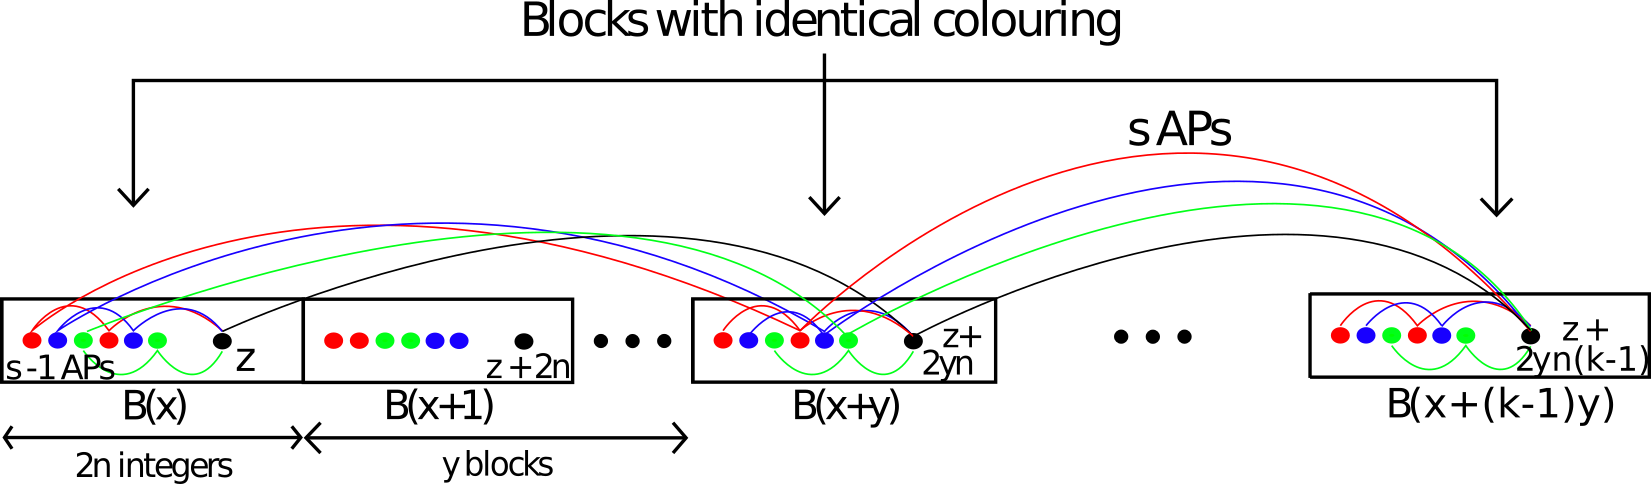
\includegraphics[scale=0.38]{Figuras/Van-der-Waerden-Blocks.png}
     \caption{s APs in the $W(r^{2n},k-1)$ blocks.}
     \label{fig:VanderWaerdenBlocks}
\end{figure}

The theorem follows from the claim by setting $s=r$ because if we have $s$  APs $\textit{colour-focused}$ at $z+2yn(k-1)$ and there is no other different colour to use in $z+2yn(k-1)$, by the fact every AP has length $k-1$  independently of the colour we choose for $z$ we will have an AP of length $k$.
\end{proof}



\chapter{Extremal Graph Theory}
In this chapter the problems and theorems are centered in extremal graphs. It embraces questions about the maximum or minimum size of a graph at the same time it satisfies certain properties.

\section{Turán's Theorem}
In this section we study forbidden subgraphs and at first we shall answer the following 
question: 
\begin{center}``What is the maximum number of edges in a tringle-free graph?''\end{center}

Note that the complete bipartite graph has $\frac{n^{2}}{4}$ edges and no triangles. The next theorem shows us this edge number is the maximum possible in a triangle-free graph.\\

\begin{theorem}[{Mantel's Theorem \cite{Ma07}}]\label{the:mantel}
If G is a triangle-free graph on $n$ vertices, then 
$$e(G) \leq \left\lceil \frac{n}{2} \right\rceil \left\lfloor \frac{n}{2} \right\rfloor .$$
\end{theorem}
\begin{proof}
This proof follows by induction on $n$. Let $G'$ be the graph obtained from $G$ by removing two vertices $u,v \in G$ such that $\{u,v\}\in E(G)$. Note that if $G$ is triangle-free, then $G'$ is also triangle-free because it is not possible to form a triangle by removing an edge and there are at most $n-1$ edges incident to $u$ or $v$, then:
\begin{align*}
e(G') &\leq \left(\left\lfloor \frac{n}{2} \right\rfloor -1\right)\left(\left\lceil \frac{n}{2} \right\rceil -1\right) \\
&= \left\lfloor \frac{n}{2} \right\rfloor \left\lceil \frac{n}{2} \right\rceil - n +1.
\end{align*}
Therefore, $e(G) \leq e(G') + n-1 = \left\lfloor \frac{n}{2} \right\rfloor \left\lceil \frac{n}{2} \right\rceil$. 
\end{proof}

Turán generalized Theorem \ref{the:mantel} in 1941 and this result will require the following definitions: 
\begin{definition}$T_r(n)$ is the complete $r$-partite graph with $n$ vertices and $\left\lceil \frac{n}{r} \right\rceil$ or $\left\lfloor \frac{n}{r} \right\rfloor$ vertices in each part.
\end{definition}

\begin{definition}
$t_r(n)$ is the number of edges in $T_r(n)$. Note that $e(T_r(n)) = t_r(n)$.
\end{definition}

\begin{theorem}[{Turán's Theorem \cite{Tu41}}] \label{theorem:turan1941}%(Turán, 1941).
If $G$ is a graph with $n$ vertices, then $$\ex(n, k_{r+1}) = t_r(n).$$
\end{theorem}

\begin{proof}
This proof follows by induction on $n$. Note $d(v) \approx n-(n/r)$ with $v \in V(G)$ and $G$ being the complete $r$-partite graph. Now, using the fact $\sum_{v\in V(G)} d(v) = 2 e(G)$ we have:

$$ t_r(n) \approx \frac{n}{2}\left(n-\frac{n}{r}\right) \approx \left(1-\frac{1}{r}\right) \binom{n}{2}.$$


 Let $e(G)$ be maximum while $G$ is a $K_{r+1}$-free graph. Construct a graph $G'$ by removing a $K_r$ from $G$ as shown in Figure \ref{fig:G'andKr}. Note that each vertex in $G'$ could be neighbour of at most $r-1$ vertices in $K_r$, otherwise $G$ would have a $K_{r+1}$, then we have $(r-1)(n-r)$ vertices between $G'$ and $K_r$.
 
 \begin{figure}[H]
     \centering
     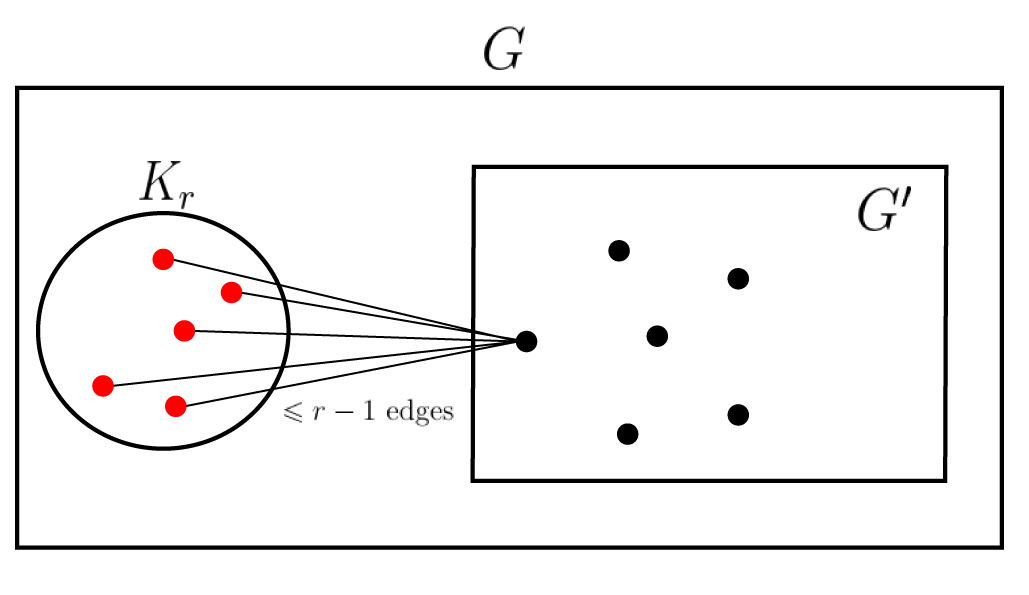
\includegraphics[scale=1]{Figuras/Kr+1-livre-prova-turan.jpg}
     \caption{$G'$ and $K_r$.}
     \label{fig:G'andKr}
\end{figure}

Note that inside the $K_r$ there exist $\binom{r}{2}$ edges and by the induction hypothesis we have $e(G') \leq t_r(n-r)$. Then it follows that:

\begin{align*}
e(G) &\leq e(G') + (r-1)(n-r) + \binom{r}{2}\\
&\leq t_r(n-r) +(r-1)(n-r) + \binom{r}{2}\\
&= t_r(n).
\end{align*}

The last line follows from the fact that $t_r(n) - t_r(n-r) = \binom{r}{2} + (r-1)(n-r)$ as we can see in Figure \ref{fig:t(n)-and-t(n-r)} removing a vertex from each partition $\{1,...,r\}$ we remove $\binom{r}{2}$ edges between the $r$ vertices removed and $(r-1)(n-r)$ edges  because every vertex in $T_r(n)$ is connected exactly with $r-1$ vertices of the $r$ removed vertices.   

 \begin{figure}[H]
     \centering
     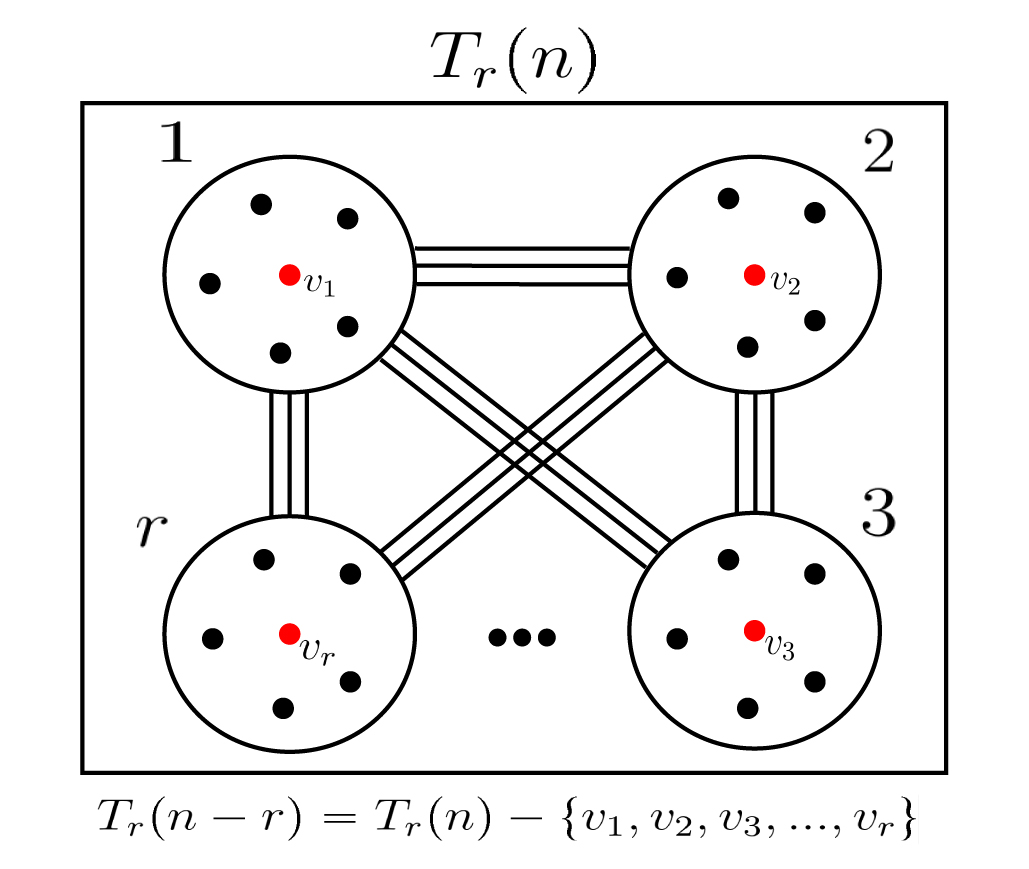
\includegraphics[scale=1]{Figuras/t(n)-and-t(n-r)}
     \caption{$T(n)$ and $T(n-r)$.}
     \label{fig:t(n)-and-t(n-r)}
\end{figure}
Then the proof is finished.
\end{proof}

\begin{theorem}[{Erd\H{o}s \cite{Er70}}]\label{theorem:erdos1970} There is an $ r$-partite graph $H$ with $V(H) = V(G)$ such that $d_H(v) \geq d_G(v)$ for every $v \in V(G)$.\\
\end{theorem}

\begin{proof}
The proof follows by induction on $r$. Let $G$ be a $ K_{r+1}$-free graph on $n$ vertices and let $w$ be a vertex of maximum degree in $G$. For every vertex $v \in V(G)\setminus N(w)$ we remove the edges incident to $v$ and add an edge between $v$ and each neighbor of $w$, this operation is called `Zykov symmetrization'. Clearly, no vertex degree has decreased because at this point $d(v) = \Delta(G)$ for every $v \in V(G)\setminus N(w)$ and the graph is still $K_{r+1}$-free because $N(w)$ has not changed and the $G\setminus N(w)$ now is an independent set.

Being $w\in V(G)$ a vertex of maximal degree in $G$, note that $H=G[N(w)]$ must be $K_r$-free by our graph choice (otherwise $G$ would not be $K_{r+1}$-free). By the induction hypothesis, exists a $(r-1)$-partite graph $H_1$ on $N(w)$ with $d_{H_1}(v) \geq d_{H}(v)$ for every $v \in N(w)$. Let $G_1$ be the graph obtained from $G$ by performing Zykov symmetrization at vertex $w$. Now replace $H$ by $H_1$ and we acquire $G_1$ which is the required $r$-partite graph, note it is valid because in any step the degrees have decreased.
\end{proof}
This theorem is related to Theorem \ref{theorem:turan1941}. In fact, Theorem \ref{theorem:erdos1970} is stronger than Theorem \ref{theorem:turan1941} and we can see this relation as follows: $$e(G) \leq e(H) \leq e(T_r(n)).$$
\section{Forbidden Bipartite Subgraphs}
In this section we study what are the consequences when small bipartite graphs are forbidden and we start with Jensen's inequality for convex functions because its importance for proving the Theorem \ref{theorem: Erdos,1938}.
\begin{proposition}[{Jensen's Inequality \cite{Je06}}]\label{prep:jensen}
 If $0\leq \lambda_i \leq 1, \sum_{i=1}^n \lambda_i = 1$ and $f$ is convex, then:

$$
f \left( \sum_{i=1}^n \lambda_i x_i\right) \leq \sum_{i=1}^n \lambda_i f (x_i).
$$

\end{proposition}

As showed in previous section, thus Theorem \ref{theorem:turan1941}:
$$ \ex (n,K_{r+1}) = e(T_{r,n}) \approx \left( 1-\frac{1}{r}\right) \binom{n}{2} .$$

Erd\H{o}s proved that the extremal number is much smaller for the $4$-cycle graph.
 
\begin{theorem}[{Erd\H{o}s \cite{Er38}}] \label{theorem: Erdos,1938} Let $G$ be a graph with $n$ vertices, then
$$\ex(n,C_4) = O(n^{3/2}).$$
\end{theorem}

\begin{proof}
A $C_4$ is formed by two `cherries' in the same pair of vertices. Counting these triples (x,\{y,z\}) of distinct vertices in $G$ such that $xy, xz \in E(G)$ and using Proposition \ref{prep:jensen} with $\lambda_i = 1/n$ we obtain the following very useful inequality,

$$ \sum_{i=1}^n \frac{1}{n} f\left(x_i\right) \geq f\left(\sum_{i=1}^n \frac{1}{n} x_i\right).$$

Applying it we have,
$$ \frac{\sum_{i=1}^n \binom{x_i}{2}}{n} \geq \binom{\frac{\sum_{i=1}^n x_i}{n}}{2} ,$$
replacing $x_i$ and assuming $\sum_{v \in V(G)} d(v) = 2e(G),$

\begin{align*}
\sum_{v \in V(G)} \binom{d(v)}{2} &\geq n \binom{\frac{2e(G)}{n}}{2}\\
&= n\frac{\frac{2e(G)}{n}\left( \frac{2e(G)}{n}-1\right)}{2} \\
&\geq \frac{n}{2} \left( \frac{2e(G)}{n} - 1 \right)^2.
\end{align*}

Since the maximum number of such triples in a $C_4$-free graph is at most $\binom{n}{2}$ because we can have only one cherry for each pair of vertices,
$$ \frac{n}{2}\left(\frac{2e(G)}{n} - 1\right)^2 \leq \binom{n}{2},$$
we obtain $e(G) = O(n^{3/2})$ finishing the proof.
\end{proof}

%Let $A = \{a_1,...,a_t\} \subset [n]$ be such that $a_ia_j \neq a_ka_l$ unless $\{i,j\} = \{k,l\}$. How big can be $A$ with these properties?
%To show a easy lower bound it is necessary only a example that fits the problem, for this problem we can use the number of primes in $[n]$ which is $\pi (n)$. But is it close to the maximum possible size?

%Erdos used theorem \ref{theorem: Erdos,1938} to answer this question.

%\begin{corollary}(Erd\H{o}s, 1938). Let $A\subseteq [n]$ be a multiplicative Sidon set. Then,
%$$ |A| \leq \pi(n) + O(n^{3/4}). $$

%\end{corollary}
The next result is very similar to theorem \ref{theorem: Erdos,1938}. In fact, it is a generalization of Erd\H{o}s' result, but instead counting cherries we count stars.
\begin{theorem}[{Kovari-Sós-Turán \cite{KoSoTu54}}]
If $G$ is a graph with $n$ vertices and $s \leq t$, then
$$ \ex(n, K(s,t)) = O (n^{2 - 1/s}). $$
\end{theorem}

\begin{proof}

For this proof we do a simple double counting on stars, which are graphs with one central vertex with a fixed number of neighbours as you can see at Figure \ref{fig:generalizedcherry}:

\begin{figure}[!htb]
     \centering
     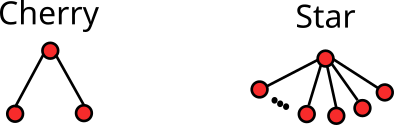
\includegraphics[scale=1]{Figuras/cherry-and-star.png}
     \caption{Cherry and Star.}
     \label{fig:generalizedcherry}
\end{figure}

$K_{1,s}$ is the star we need to count. Note we can count it by taking all possible sets of $s$ neighbours of each vertex, as follows,
$$ |\{K_{1,s}\colon K_{1,s} \subseteq G\}| = \sum_{v \in V(G)} \binom{d(v)}{s} .$$

Now we use the fact $\left(\frac{n}{m}\right)^m \leq \binom{n}{m} \leq \left(\frac{en}{m}\right)^m$ and Jensen's Inequality \ref{prep:jensen} to acquire the following inequality,

\begin{align*} 
\sum_{v \in V(G)} \binom{d(v)}{s} & \geq n\binom{\sum_{v \in V(G)} d(v)/n}{s}\\ 
& \geq \frac{1}{s^s} n \left( \frac{\sum_{v \in V(G)} d(v)}{n} \right) ^s \\
& = \frac{1}{s^s} n \left( \frac{ 2 e(G)}{n} \right) ^s \\
& = c(s) \frac{e(G)^s}{n^{s-1}},
\end{align*}
where $c(s) = \left(2/s\right)^s$.
We already have a lower bound for $K_{1,s}$ that depends of the number of edges, now let's construct a upper bound counting the maximum number of generalized cherries.
As $K(s,t)$ is the complete bipartite graph with two partitions whose sizes are $|s|$ and $|t|$ we know the maximum number of $K_{1,s}$ is $t\binom{n}{s}$ but since we want the maximum number of edges in $G$ without a $K_{s,t}$ we have,

\begin{align*}
c(s) \frac{e(G)^s}{n^{s-1}} &\leq |\{K_{1,s}\colon K_{1,s} \subseteq G\}|\\
&\leq (t-1) \binom{n}{s}\\
		       & \Rightarrow e(G)^s \leq \frac{1}{c(s)}\frac{e^s(t-1)}{s^s}n^{2s-1}\\
		       &\Rightarrow e(G) \leq c(s,t) n^{2-1/s}\\
		       &\Rightarrow e(G) = O(n^{2-1/s}),
\end{align*}
where $c(s,t)= \sqrt[s]{\frac{1}{c(s)}\frac{e^s(t-1)}{s^s}}$ . Using again the fact $\binom{n}{m} \leq \left(\frac{en}{m}\right)^m$ we have what we want to show and the proof is finished.
\end{proof}

%\section{The Erd\H{o}s-Stone Theorem}
%This theorem is extremely important for graph theory and can be called as the fundamental theorem of graph theory such its importance. To prove it we need the following definition.
%\begin{definition} The Chromatic Number:
%$$\chi(G) = \text{ min}\{r: \exists c : V(G) \rightarrow [r] \text{ such that } c(u) \neq c(v) \text{ for every } uv \in E(G)\}$$ 
%\end{definition}

%Note $\chi(G)$ is related to $r$-partite graphs, a graph $G$ is $r$-partite if and only if $\chi(G) \leq r$.


%\begin{theorem}
%(Erd\H{o}s and Stone, 1946). Let H be an arbitrary graph. Then
%$$ ex(n,H) = \left(1-\frac{1}{\chi (H)-1} + o(1)\right) \binom{n}{2}.$$ 
%\end{theorem}

%\begin{proof}

%Here will be the proof.

%\end{proof}

\chapter{Random Graphs}
\section{The Probabilistic Method}
This method has incredible simple applications, when this method begun to being used it created many shocking proofs, but not all applications of the method are so simple or easy to understand. A central fact for the simpler version of the probabilistic method is ``a object with property $ A$ exists $\iff  \mathbb{P}(\text{object has property }A)>0$''.

It is necessary to introduce the Erd\H{o}s-Rényi random graph model $G(n,p)$. $G(n,p)$ is a probability distribution on graphs, more informally, it is an edge distribution on $n$ vertices with probability $p$ and with the existence of edges being independent events.

\begin{definition}\label{def:randomgraph}
The (Erd\H{o}s-Rényi) random graph $G(n,p)$ is the graph on $n$ vertices obtained by choosing each edge independently and uniformily at random with probability $p$. In other words, we assume that we have a probability space $\Omega$ and independent random variables $I_{vw}$ for each $\{v,w\} \in \binom{[n]}{2}$, such that
$$\mathbb{P}(I_{vw} = 1) = 1 - \mathbb{P}(I_{vw} = 0),$$ 
and let $G$ be the graph with vertex set $[n]$ and edge set $\{\{v,w\} \in \binom{[n]}{2}: I_{vw} = 1\}$. 

\end{definition}

%$$\mathbb{P}(e \in E(G(n,p)))=p ,$$ \\and\\$$ 1-p=\mathbb{P}(e \notin E(G(n,p))),$$

%{\bf Question:} What is the probability of $G(n,p) = H$, with $H$ being a fixed graph?
%Intuitively we can guess there exists a really small chance that this event occurs and the intuition in this case is true, let's see this probability below,
%$$\mathbb{P}(G(n,p)=H) = p^{e(H)}(1-p)^{\binom{n}{2}-e(H)}.$$

The next theorem \ref{erdoss} introduces the method and it is presented two different proofs, being the second one smaller. In order to prove it we will need the following definitions.

\begin{definition}\label{def:girth}
$g(G)$ is the girth of $G$ which is the length of the shortest cycle in $G$. 
\end{definition}
\begin{definition}\label{def:independencenumber}
$\alpha(G) = \max\{|A|: A$ is an independent set$\}$.
\end{definition}
\begin{definition}\label{def:chromaticnumber}
$\chi(G)$ is the minimum number of colours used in a proper colouring of G.
\end{definition}
Assuming $\chi(G(n,p)) = r$ we have a $\{V_1,V_2,...,V_r\}$ partition of $V(G(n,p))$ on $r$ independent sets illustrated at Figure \ref{fig:r-partition}


\begin{theorem}\label{erdoss}[{Erd\H{o}s \cite{Er59}}] There exist graphs whose girth and chromatic number are arbitrarily large.
\end{theorem}

\begin{proof} 1.
We will prove that:

$$\mathbb{P}(\chi(G(n,p)) \geq k \text{ and } g(G(n,p)) \geq k) > 0 ,$$
for some $p =p(n) \in (0,1)$ and a sufficiently large $n$.

Assuming $\chi(G(n,p)) = r$ we have a partition $\{V_1,V_2,...,V_r\}$ of $V(G(n,p))$ on $r$ independent sets illustrated in Figure \ref{fig:r-partition}.
 
\begin{figure}[!htb]
     \centering
     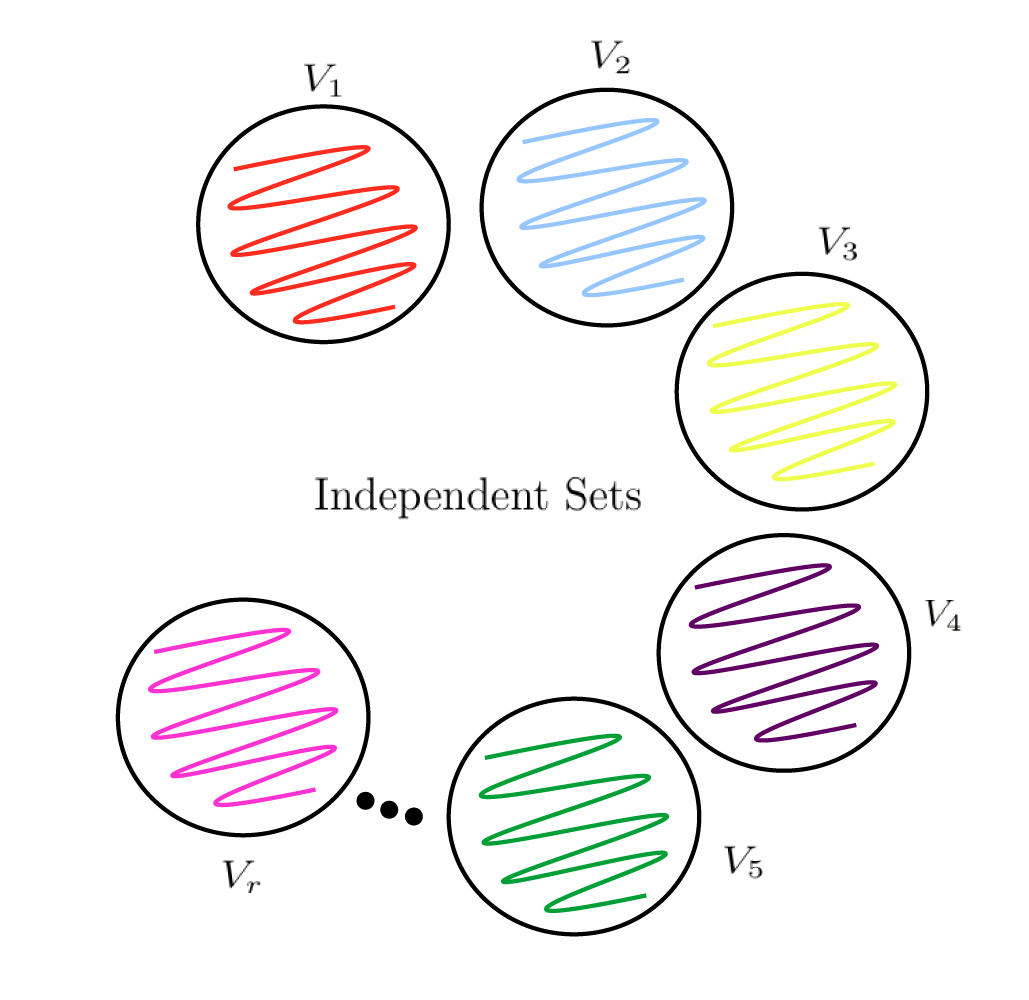
\includegraphics[scale=1]{Figuras/r-partion.jpg}
     \caption{r-colouring partition. }
     \label{fig:r-partition}
\end{figure}

Then, $\alpha (G(n,p)) \geq \frac{n}{r}$ and since $\chi(G)=r$,

$$\chi(G(n,p)) \geq \frac{n}{\alpha(G(n,p))},$$
and we want to show that

$$\chi(G(n,p)) \geq \frac{n}{\alpha(G(n,p))} \geq k ,$$
then,

$$\alpha(G(n,p)) < m \iff X_m=0 ,$$
where 
%$X_m = \{|[A]|: S \in A$ if $S$ is a independent set with at least $m$ elements in $G(n,p)\}$,
$X_m = \big|\{S\in V(G(n,p))\colon \text{$S$ is an independent set with exactly $m$ vertices in $G(n,p)$}\}\big|$,
and follows $m = \frac{n}{k}$. 
\begin{align*}
\mathbb{E}[X_m]&=\sum_{\substack{S \in V(G) \\ |S| = m}} \mathbb{P}(S\text{ is independent})\\
&=(1-p)^{\binom{m}{2}} \binom{n}{m}.
\end{align*}

Since  $\left(\frac{n}{m}\right)^m \leq \binom{n}{m} \leq \left(\frac{en}{m}\right)^m$ and $1-x \leq e^{-x}$, we obtain that
\begin{align*}
\mathbb{E}[X_m] &\leq \left(\frac{en}{m}\right)^m  e^{(-pm^2)} \\
&= \left(\frac{en}{m} e^{(-pm)}\right)^m\\
%&\leq \left(\frac{en}{m} e^{(-pm)}\right)^m \\
&= \left(\frac{en}{m}\frac{1}{e^{(pm)}}\right)^m  \\
&\ll 1.
\end{align*}

Note that we need $e^{pm} \gg n$ and recall that $m =\frac{n}{k}$ then isolating $p$ we have

$$ pn/k \gg \log n \Rightarrow p \gg \frac{k\log n}{n},$$
by Markov's inequality,
 
 $$ \mathbb{P}(X_m \geq 1) \leq \mathbb{E}[X_m] ,$$
 
and if $p \gg \frac{k \log n}{n}$ we have,
 
 \begin{align*}
\mathbb{P}(X_m \geq 1) &\leq \mathbb{E}[X_m] \\
&\leq \frac{1}{100}  \\
&\Rightarrow \mathbb{P}\left(\alpha (G(n,p)) < \frac{n}{k}\right) \geq \frac{99}{100}\\ 
&\Rightarrow  \mathbb{P}\left(\chi(G(n,p)) > k \right) \geq \frac{99}{100}.
\end{align*}

Since the proof for $\chi(G) \geq k$ is finished we will prove $g(G(n,p))\geq k$,

$$ g(G(n,p)) \leq k \iff X_k \geq 1,$$
where $X_k = |C_k \colon C_k \subseteq G(n,p)|$,

$$\mathbb{E}[X_k] = \sum_{C_k \subseteq K_n} \mathbb{P}(C_k \subseteq G(n,p) ) \leq n^kp^k.$$

Now we need to limit our short cycles by $\sqrt{n}$ in order to show with high probability we will have few short cycles so we can destroy them,

$$n^kp^k \leq \sqrt{n} \text{ if } p \leq n^{-1 + \frac{1}{2k}},$$
then getting together with our previous result,

$$\frac{k\log k}{n} \ll p \leq n^{-1 + \frac{1}{2k}}.$$

We can remove a vertex of each cycle with length $<k$, so we have $g(G) \geq k$. Note that removing a cycle's vertex does not make $\alpha(G)$ bigger and consequently does not make $\chi(G)$ smaller, maintaining all our previous calculations valid.
\end{proof}

\begin{proof}2.
We have,

$$ |V(G)| = \sum_{i=1}^{\chi(G)} |S_i| \leq \chi(G)\max|S_i| \leq \chi(G) \alpha (G) .$$

Note that if $\alpha(G) \leq |G|/k$, then $\chi(G) \geq $k. Let $\varepsilon > 0$ be sufficiently small ($\varepsilon < 1/k$) and $p = n^{\varepsilon - 1}$. As we have already introduced to $G(n,p)$ in definition \ref{def:randomgraph} let $G = G(n,p) $.% $-$\{one vertex of each cycle $C_{\ell} \text{ with } \ell\leq k\}$.

Now we need two claims to reach the result. We claim that, with high probability, $G$ has at most $n/2$ cycles of length $\leq k$ and has no independent set  of size $n/2k$ then, consequently $\chi(G) \geq k$ and $girth(G) \geq k$.

First claim. $V(G) > n/2$ . First of all we need some variables to count the cycles,
$$X_{\ell} =  |C_{\ell} : C_{\ell} \subseteq G(n,p)|$$
$$X = \text{quantity of short cycles } = \sum_{{\ell}=3}^k X_{\ell}$$
\begin{align*}
\mathbb{E}[X] &= \sum_{{\ell}=3}^k \mathbb{E}[X_{\ell}] \\
	       &= \sum_{{\ell}=3}^k \sum_{C_{\ell} \in K_n} \mathbb{P}(C_{\ell} \subseteq G(n,p))\\
	       &\leq \sum_{{\ell}=3}^k n^{\ell} p^{\ell} \\
	       &= \sum_{{\ell}=3}^k n^{\varepsilon {\ell}}\text{, with } p= n^{\varepsilon - 1}\\
	       &\leq 2n^{\varepsilon k} \\
	       &= o(n).
\end{align*}

Note that since we are removing a vertex of each cycle $V(G) \geq n-X$. Now we show the general case for this useful inequality for the probabilistic method. The Markov's inequality holds for any random variable which takes non-negative values and for $a>0$,

$$\mathbb{P}(X>a) \leq \frac{\mathbb{E}(X)}{a}.$$

Using it and replacing $\mathbb{E}[X]$ by its upper bound we have,

\begin{align*}
\mathbb{P}(X\geq n/2) &\leq \frac{\mathbb{E}[X]}{n/2}\\
		& = o(n)/n\\
		& = o(1).
\end{align*}

Then, we proved that, with high probability, the graph do not have more than $n/2 -1$ cycles with length at most $k$ and consequently we have $|V(G)| > n/2$ .

Second claim. $\alpha(G) \leq \alpha (G(n,p)) < n/2k$. We need to count the independent sets
$$Y_{\ell} = \text{quantity of independents sets with length ${\ell}$. }$$

\begin{align*}
\mathbb{E}[Y_{\ell}] &= \sum_{\substack{|S| = {\ell} \\ e(S) = 0 }} (1-p)^{\binom{{\ell}}{2}}\\
	       &= (1-p)^{\binom{{\ell}}{2} \binom{n}{{\ell}}} \\
	       &\leq \left(\frac{en}{{\ell}}\right)^{\ell} e^{-p\binom{{\ell}}{2}}\\
	       &\rightarrow 0,
\end{align*}
if $\ell = n/2k$. Thus we have

$$\frac{\mathbb{E}[|\{C_{\ell} \subseteq G : {\ell}\leq k \}|]}{n/2} + \mathbb{E} [|\{ S:|S| \geq n/2k, e(S) = 0\}|] \rightarrow 0$$
as $n \rightarrow \infty $. So $G$ has the desired properties with high probability and the proof is finished.
\end{proof}

Realize that the key point in both proofs was the fact we could choose the most comfortable probability distribution, what gives us a huge flexibility to construct proofs.

\section{Subgraphs of the Random Graph}

In this section we will manipulate $p$ in order to have a specific subgraph contained in $G$. Being more specific we shall prove the threshold for the property ``containing a triangle'' in $G$.  We will need the Chebychev inequality presented below.

\begin{theorem}[{Chebyshev's Inequality \cite{Ch67}}]
$$\mathbb{P}(|X-\mu| \geq a) \leq \sigma^2/a^2.$$
\end{theorem} 

Using $a = \mu$, we have the following very useful inequality,

$$\mathbb{P}(X=0) \leq \mathbb{P}(|X-\mu | \geq \mu) \leq \sigma^2/\mu^2,$$
which gives us an upper bound for $\mathbb{P}(X=0)$. We shall use it to prove the following result.\\

\begin{theorem}
Let $G=G(n,p)$ be a random graph.
Then,
$$
\mathbb{P}(G\text{ contains a triangle}) \rightarrow 
\begin{cases}
		0, &\text{if $p\ll 1/n$},\\
		1, &\text{if $p\gg 1/n$}\,.
\end{cases}
$$
\end{theorem}

\begin{proof}
In the first part we need the random variable and  Markov's inequality as follows,
$$ X = \text{ the quantity of triangles in } G.$$
\begin{align*}
\mathbb{P}(G\text{ contains a triangle}) &\leq \mathbb{E}(X)\\
& \leq \binom{n}{3}p^3 \\
& \ll 1,
\end{align*}
if $ p \ll 1/n$, finishing the first part of the proof. To prove the second part we need to bound the variance of the random variable.

\begin{align*}
Var(X) &= \mathbb{E}(X^2) - \mathbb{E}(X)^2\\
& = \mathbb{E} \left( \sum_{(u, v)} \mathbbm{1}[u]\mathbbm{1}[v] \right) - \left( \sum_u \mathbb{P}(u) \right) ^2\\
& = \sum_{u,v} \left(\mathbb{P}(u \wedge v) - \mathbb{P}(u)\mathbb{P}(v)\right),
\end{align*}
where $v$ and $u$ denote the events that specific triangle occurs and the $\mathbbm{1}$ denotes the indicator function, assuming value $1$ if the event occurs and $0$ otherwise. Note that the pairs $u,v$ which are independent appear in both terms as follows

\begin{align*}
Var(X) &= \sum_{u,v} \left(\mathbb{P}(u \wedge v) - \mathbb{P}(u)\mathbb{P}(v)\right)\\
%& = \sum_{|u \cap v| = 0}\left( \mathbb{P}(u \wedge v) - \mathbb{P}(u)\mathbb{P}(v)\right)\\ &+ \sum_{|u \cap v| = 1}\left( \mathbb{P}(u \wedge v) - \mathbb{P}(u)\mathbb{P}(v)\right)\\ &+ \sum_{|u \cap v| = 2}\left( \mathbb{P}(u \wedge v) - \mathbb{P}(u)\mathbb{P}(v)\right)\\ &+ \sum_{|u \cap v| = 3}\left( \mathbb{P}(u \wedge v) - \mathbb{P}(u)\mathbb{P}(v)\right)\\
& \leq \sum_{|u \cap v| = 2}\mathbb{P}(u \wedge v) + \sum_{|u \cap v| = 3}\mathbb{P}(u \wedge v)\\
&\leq n^4 p^5 + n^3 p^3,
\end{align*}
%$$ \sum_{|u \cap v| = 1}\mathbb{P}(u \wedge v)   = n^5p^5$$
and using Chebychev's inequality,
$$\mathbb{P}(G \text{ contains no triangles}) \leq \frac{Var(X)}{\mathbb{E}(X)^2} \leq \frac{n^4p^5 + n^3p^3 }{n^6p^6} \ll 1,$$
for $p \gg 1/n$, finishing the proof.
 \end{proof}

\section{The Janson and FKG Inequalities}

In this section we focus on the occurrence of  bad events, asking questions as the form ``Could we count the number of bad events?'' or ``What is the probability that none of the bad events occurs?''. The Janson and FKG inequalities give us tools to answer this type of questions.

\subsection{The FKG Inequality}
In this subsection we shall use FKG inequality to acquire an upper bound for Theorem \ref{theo:FKG}, but first we introduce some concepts and present the FKG inequality.

\begin{definition}
Monotone Increasing. Let $\mathcal{A}$ be a collection of graphs on $n$ vertices, $\mathcal{A}$ is monotone increasing if $G \in \mathcal{A}$ and $e(G) \subseteq e(H)$ implies $H \in \mathcal{A}$, so if $G \in \mathcal{A}$ this means adding edges does not make $G$ loose the characteristics that makes it be in $\mathcal{A}$ and it is called monotone decreasing otherwise.     
\end{definition}

\begin{example}
``$G$ contains a triangle'' is monotone increasing because it is impossible to destroy a triangle adding edges.
\end{example}

\begin{theorem} [{FKG Inequality \cite{FKG71}}]
 Let $\mathcal{A}$ and $\mathcal{B}$ be monotone increasing and let $\mathcal{C}$ be monotone decreasing, then:

$$ \mathbb{P}((G(n,p) \in \mathcal{A}) \wedge (G(n,p) \in \mathcal{B})) \geq \mathbb{P}(G(n,p) \in \mathcal{A})\mathbb{P}(G(n,p) \in \mathcal{B}),$$
and
$$ \mathbb{P}((G(n,p) \in \mathcal{A}) \wedge (G(n,p) \in \mathcal{C})) \leq \mathbb{P}(G(n,p) \in \mathcal{A})\mathbb{P}(G(n,p) \in \mathcal{C}).$$
\end{theorem}

FKG inequality presented follows the theorem we want to prove.
\begin{theorem} \label{theo:FKG}
Let $c$ be a constant and $p = \frac{c}{n}$. Then

$$ \limsup_{n \rightarrow \infty}\mathbb{P}(G(n,p)\text{ contains a triangle }) = 1 - e^{\frac{-c^3}{6}}.$$
\end{theorem}
\begin{proof}

We start using FKG inequality to prove the upper bound.\\
Let $X$ be a triple in $[n]$ and $B_X$ be the event that this triple forms a triangle in $G_n,p$. Note that the events $\overline{B_X}$ are monotone decreasing and have probability $(1-p)^3$.

\begin{align*}
\mathbb{P}(G(n,p) \text{ has no triangles }) &= \mathbb{P}\left( \bigwedge_{X \in \binom{[n]}{3}} \overline{B_X}\right) \\
& \geq \prod_{X \in \binom{[n]}{3}} \mathbb{P}(\overline{B_X})\\
& \geq (1-p^3)^{\binom{n}{3}}\\
& \rightarrow e^{-\mathbb{E}[X]}\\
& = e^{-c^3/6},
\end{align*}
as $n \rightarrow \infty$ finishing the upper bound proof. For the lower bound proof we shall use same definition of $X$ and $B_X$ used before. Thus we have a set of $\binom{n}{3}$ events $B_X$ of the form $A_X \subseteq E(G(n,p)) \subseteq \binom{n}{2}$.
Note that 
$$\mu = \sum_X \mathbb{P} (B_X) = p^3\binom {n}{3},$$
and
$$\Delta = \sum_{X\sim Y} \mathbb{P}(B_X \wedge B_Y) = O(n^4 p^5) \ll 1.$$

Then using the Janson's inequality 

$$ \mathbb{P}\left(\bigwedge_{j=1}^m \overline{B_j}\right) \leq e^{-\mu + \Delta/2}, $$
which we shall prove next we have the following 
$$ \mathbb{P}(G(n,p)\text{ has no triangles }) \leq e^{-\mu + \Delta/2} \rightarrow e^{-c^3/6}$$
as $n \rightarrow \infty$, finishing the proof.
\end{proof}

\subsection{Janson's Inequality}

In this subsection we shall use Janson's inequalities to prove the bound given by the FKG inequality is sharp under certain circumstances.

Let $A_1, ... , A_m$ be subsets of $[N]$ and $Y$ be a set in $[N]$ whose elements are chosen independently, with $\mathbb{P}(j \in Y) = p$ for each $j$ and $N=\binom{n}{2}$. 

$$ B_j = \{A_j \colon A_j \subseteq Y\},$$
note that the events are monotone increasing and that $B_i$ and $B_j$ are independent $\iff A_i \cap A_j \neq \emptyset$. 

Define $\mu = \sum_j \mathbb{P}(B_j)$ denoting the expected number of bad events and let

$$ \Delta = \sum_{\substack{i\sim j\\ (i,j) \in [N]^2}} \mathbb{P}(B_i \wedge B_j), $$
where the sum is over ordered pairs $(i,j)$ such that $A_i$ and $A_j$ intersect. Follows the Janson inequalities.

\begin{theorem}[{Janson's Inequality \cite{Ja87}}]
Let $A_1,...,A_m \subseteq [n]$ and let $B_1,...,B_m$ be the events defined above. Then

$$ \mathbb{P}\left(\bigwedge_{j=1}^m \overline{B_j}\right) \leq e^{-\mu + \Delta/2}. $$

And if $\Delta \geq \mu$, then

$$ \mathbb{P}\left( \bigwedge_{j=1}^m \overline{B_j} \right) \leq e^{-\mu ^2 /2\Delta}.$$
\end{theorem}
By FKG inequality we have,

$$ \mathbb{P}\left( \bigwedge_{j=1}^m \overline{B_j} \right) \geq \prod_j (1-\mathbb{P}(B_j)) \approx e^{-\mu}, $$
if $\mathbb{P}(B_j) \ll 1$ for each $j$, so the Janson inequalities are close to being sharp.We shall prove the first inequality.

\begin{proof}
We claim that, for each $j \in [m]$,

$$\mathbb{P} \left( B_j | \bigwedge_{i=1}^{j-1} \overline{B_i} \right) \geq \mathbb{P}(B_j) - \sum_{i\sim j, i<j} \mathbb{P}(B_i \wedge B_j). $$

In order to prove the claim we need to divide the event $\bigwedge^{j-1}_ {i=1} \overline{B_i}$ into two parts, $E$ and $F$. Let $E$ denote the event $\bigwedge_{i \in I} \overline{B_i}$, where

$$ I = \{ i \in [j-1]: i \sim j \},$$
(i.e., the set of indices $i$ such that $A_i \cap A_j$ is non-empty), and let $F$ denote the event $\bigwedge_{i \in J} \overline{B_i}$, where $J=[j-1]\backslash I$. Note that the event $B_j$ is independent of the event $E$, and that $E$ and $F$ are both monotone decreasing. By the FKG inequality,

\begin{align*}
\mathbb{P}(B_j | E \cap F) & \geq \mathbb{P}(B_j \wedge E | F)\\
& = \mathbb{P}(B_j | F) \mathbb{P}(E | B_j \wedge F)\\
& \geq \mathbb{P}(B_j)\mathbb{P}(E|B_j)\\
& \geq \mathbb{P}(B_j) - \mathbb{P}(B_j) \mathbb{P}(\overline{E} | B_j)\\
& \geq \mathbb{P}(B_j) - \sum_{i \sim j, i < j}\mathbb{P}(B_j) \mathbb{P}(B_i | B_j).
\end{align*}

Since the claim is proved, note that, from $\mathbb{P}(A\cap B) = \mathbb{P}(A)\mathbb{P}(B|A)$ we have,

\begin{align*}
\mathbb{P}\left( \bigwedge_{j=1}^m \overline{B_j} \right) &= \prod_{j=1}^m \mathbb{P}\left( \overline{B_j} | \bigwedge_{i = 1}^{j-1} \overline{B_i}\right)\\
& = \prod_{j=1}^m \left( 1 - \mathbb{P}\left(B_j | \bigwedge_{i = 1}^{j-1} \overline{B_i}\right)\right)\\
& \leq \exp\left(- \sum_{j=1}^m \mathbb{P}(B_j | \bigwedge_{i=1}^{j-1} \overline{B_i}\right),
\end{align*}
using the claim we just proved,
\begin{align*}
\mathbb{P}\left( \bigwedge_{j=1}^m \overline{B_j} \right) &\leq  \exp\left(- \sum_{j=1}^m \mathbb{P}(B_j) + \sum_{i \sim j, i< j} \mathbb{P}(B_i \wedge B_j)\right)\\
& = \exp( - \mu + \Delta /2).
\end{align*}

Then we finish the proof of the first inequality. Now we proceed with the proof of the second inequality, with $\Delta \geq \mu$.

$$\mathbb{P}(\bigwedge_{j=1}^m \overline{B_j}) \leq \mathbb{P}(\bigwedge_{j \in T} \overline{B_j}),$$
for all $T$ in $\binom{n}{2}$ with $T$ chosen randomly. We define $\mathbb{P}(j \in T) = q$ for all $j$ independently, then we have,

$$ \mathbb{P}(\bigwedge_{j \in T} \overline{B_j}) \leq e^{- \mu(T) + \Delta(T)/2},$$
with
 $$\mu(T) = \sum_{j \in T} \mathbb{P}(B_j),$$
 and
 \begin{align*}
 \mathbb{E} [\mu(T)] &= \sum^m_{j=1} \mathbb{P}(j\in T) \mathbb{P} (B_j)\\
& = q\mu .
 \end{align*}

And we have
 $$ \mathbb{E}[\Delta(T)] = q^2\Delta.$$
 
 Then,
 $$\mathbb{E}[\mu(T) - \Delta(T)/2] = q\mu - q^2 \Delta/2,$$
 which by the fact $\mathbb{E}[X] \geq a \Rightarrow \mathbb{P}(X\geq a) > 0$,
 $$\Rightarrow \mathbb{P}(\mu(T) - \Delta(T)/2 \geq q\mu - q^2 \Delta / 2) > 0$$
 $$\Rightarrow \exists T \subseteq \binom{n}{2}\text{ such that } \mu(T) - \Delta(T)/2 \geq q\mu - q^2 \Delta / 2 .$$
 
Now maximizing $q = \mu / \Delta \leq 1$ we have

 $$ \mu(T) - \Delta(T)/2 \geq \frac{\mu^2}{\Delta} - \frac{\mu^2}{2\Delta}$$
 $$\Rightarrow -\mu(T) + \frac{\Delta(T)}{2} \leq -\frac{\mu^2}{2\Delta}.$$
 
 Then we finish the proof.
 
\end{proof}

\section{Connectedness}
At this section we will answer the question ``For which $p$ is $G(n,p)$ likely to be connected?'' Observe this property is monotone increasing, because it is not possible to disconnect a graph by adding edges. The following theorem gives a threshold for this property.

\begin{theorem}
For every $\varepsilon > 0$,

$$
\mathbb{P}(G(n,p)\text{ is connected}) \rightarrow 
\begin{cases}
		0, &\text{ if }p \leq \frac{(1 - \varepsilon) \log n}{n},\\
		1, &\text{ if }p \geq \frac{(1 + \varepsilon) \log n}{n}\,,
\end{cases}
$$
as $n \rightarrow \infty$.
\end{theorem}
\begin{proof}
We start proving what happens when $p \leq \frac{(1 - \varepsilon) \log n}{n}$. In order to have a connected $G\colon G \in G(n,p)$ we need to avoid isolated vertices. Let $X=X(G)$ denote the number of isolated vertices in $G$ and let $p\leq((1-\varepsilon) \log n) /n$. Then using the fact $1-x > e^{-x-x^2}$,

$$ \mathbb{E}[X(G)] = n(1-p)^{n-1} > ne^{-pn-p^2n} \gg n^{\varepsilon/2},$$
for sufficiently large $n$. Now we can bound the variance of $X(G)$ as below,

\begin{align*}
Var(X) &= \mathbb{E}[X^2 ] - \mathbb{E}[X]^2\\
&= \sum_{x,y} \mathbb{P}(d_x = d_y =0) - \left( \sum_x \mathbb{P}(d_x = 0\right)^2\\
& = 2\binom{n}{2} (1-p)^{2n-3} + n(1-p)^{n-1} - n^2(1-p)^{2n-2}\\
& = (n^2 - n)(1-p)^{2n-3} + n(1-p)^{n-1} - n^2(1-p)^{2n-2}\\
& = n^2(1-p)^{2n-3}\left( \frac{n-1}{n} - (1-p) \right) + n(1-p)^{n-1}\\
& = n^2(1-p)^{2n-3}\left( -\frac{1}{n} + p \right) + n(1-p)^{n-1}\\
& = pn^2 (1-p)^{2n-3} + n(1-p)^{n-1} - n(1-p)^{2n-3}\\
& \ll n^2 (1-p)^{2n-2}\\
& = \mathbb{E}[X]^2.
\end{align*}

Then we just showed $Var(X) \ll \mathbb{E}[X]^2$ and now we can use Chebychev  inequality,

$$\mathbb{P}(X=0) \leq \mathbb{P} (X-\mathbb{E}(X) \geq \mathbb{E}(X)) \leq \frac{Var(X)}{\mathbb{E}(X)^2} \rightarrow 0.$$

We can conclude $\mathbb{P}(G\text{ is connected}) \rightarrow 0$ as $n \rightarrow \infty$ finishing the prove of the first part.

To prove the second part, we define the random variable $Y_k(G)$, which counts the number of components of size $k$ in $G$. Bounding the expected number we have

\begin{align*}
\mathbb{E}[Y_k (G)]  & \leq \sum_{\substack{S\subseteq V(G) \\ |S| = k}} \mathbb{P}(S\text{ is a component})\\
&\leq \binom{n}{k}(1-p)^{k(n-k)}\\
&\leq \left( \frac{en}{k} \right) ^k e^{-pk(n-k)}\\
& = \left( \frac{en}{k} e^{-p(n-k)} \right)^k.
\end{align*}

Note that if $G$ is not connected, there must exist a component of size at most $ n/2$ then $1 \leq k \leq n/2$. Since the function $\left( \frac{en}{k} e^{-p(n-k)} \right)$ is convex the highest value of it occurs in one of its extremal points thus we have
$$\mathbb{E}[Y_k (G)] \leq (\max\{ene^{-p(n-1)}, 2ee^{-pn/2}\})^k .$$

Note that, \\
for $ene^{-p(n-1)}$ and $p \geq \frac{(1 + \varepsilon) \log n}{n}$ we have $\mathbb{E}[Y_k (G)] \rightarrow 0$\\
and for $2ee^{-pn/2}$ and $p \geq 4/n$ we have $\mathbb{E}[Y_k (G)] \rightarrow 0$.\\

Using the maximum one we have $p \geq \frac{(1 + \varepsilon) \log n}{n}$  and by Markov's inequality

 $$\mathbb{P}(Y_k \geq 1) \leq \mathbb{E}[Y_k] \rightarrow 0,$$
 which implies $\mathbb{P}(\text{G is connected}) \rightarrow 1$, finishing the proof.

\end{proof}
\chapter{Regularity}
In this chapter we present the Szemerédi's Regularity Lemma which is a really powerful tool in Combinatorics. It give us a method to approximate any arbitrary graph to a random graph, which means any arbitrary graph can be transformed in order to share useful properties with random graphs.

\begin{example}
With at least how many edges can we say a graph $G$ has a triangle?

For arbitrary graphs:
$$ e(G) > \frac{n^2}{4} \Rightarrow G \text{ has a triangle. }$$

For random graphs:
$$ e(G) \gg n \Rightarrow G\text{ has a triangle w.h.p. } $$

As we can see random graphs give us different type of information based on probability.

\end{example}

\section{The Regularity Lemma}

Informally, the lemma says that if you partition a given graph enough then the partition pairs look random-like. Before showing the formal form we need to define $\varepsilon$-regular and to show the properties that make it looks random-like.

\begin{definition}
Given a graph $G$ and disjoint sets $A$ and $B$ of vertices, we say that $(A,B)$ is $\varepsilon$-regular if $\text{ for every } X \subseteq A \text{ and every } Y \subseteq B\text{ with } |X| \geq \varepsilon|A| \text{ and } |Y| \geq \varepsilon |B|$ we have
$$ \left| \frac{e(X,Y)}{|X||Y|} - \frac{e(A,B)}{|A||B|} \right| \leq \varepsilon  .$$
\end{definition}


A property shared between random graphs and $\varepsilon$-regular pairs is that most vertices have roughly the same number of neighbours.

\begin{fact}\label{fact:503}
Let $(A,B)$ be an $\varepsilon$-regular pair of density at least $\delta$ in a graph $G$. Then only $2 \varepsilon |A| $ vertices of $A$ have a degree out of the interval $(\delta - \varepsilon)|B| \leq d(v): v \in A \leq (\delta + \varepsilon)|B|$ in $G[A,B].$
\end{fact}
\begin{proof}
Let $X = \{v \in A \colon | N_G(v) \cap B | < (\delta-\varepsilon)|B|\}$ and let $Y=B$. Then note that the density of the pair $(X,Y)$ is at most  $\delta - \varepsilon -1$, which implies $|X| < \varepsilon |A|$, otherwise it would contradict the definition of $\varepsilon$-regular pairs. By symmetry, the same holds for $Z = \{ v \in V(A) \colon |N_G(v) \cap B| > (\delta+\varepsilon)|B|\}$. Then we have at most $2 \varepsilon |A| $ vertices of $A$ that do not have roughly the same number of neighbours.

Alternatively, we could have noticed that from the definition of $\varepsilon$-regular pairs, with $|X| \geq \varepsilon|A|, |Y|\geq \varepsilon|A|$ and $e(A,B)/|A||B| \geq \delta $, we have

$$ \frac{e(X,Y)}{|X||Y|} \geq \frac{e(A,B)}{|A||B|} - \varepsilon \geq \delta - \varepsilon,$$
let $Y = B$ then
$$ \frac{e(X,B)}{|X|} \geq (\delta - \varepsilon)|B|,$$
which corresponds to average degree of $v \in X$, confirming the claimed result.
\end{proof}

Now we prove the embedding lemma that makes the regularity useful to solve problems. It says that for the purpose of finding small subgraphs in graph $G$, dense $\varepsilon$-regular pairs can be treated as complete bipartite graphs.

%\begin{definition}
%$\mathcal{G}(H,m,\varepsilon,\delta)$ denotes the family of graphs $G$ such that $V(G) = V(H(m))$, $G\subset H(m)$, and $G[A_i,A_j]$ is $\varepsilon$-regular and has density at least $\delta$ whenever $ij \in E(H)$.
%\end{definition}

\begin{lemma}\label{lemma:embeddinglemma}
%The Embedding Lemma. Let $H$ be a graph, and let $\delta >0$. There exists $\varepsilon>0$ and $N \in \mathbb{N}$ such that if $n \geq N$ and $G \in \mathcal{G}(H,n,\varepsilon,\delta)$, then $H \subset G$.


(The Embedding Lemma - simple version). Let $H$ be a graph, and let $\varepsilon >0$. There exist $\delta >\varepsilon$ and $M \in \mathbb{N}$ such that if $m \geq M$ and there exist a partition $\{V_1, ..., V_H\}$ with all pairs being $\varepsilon$-regular and $\delta$-dense, then $H \subseteq G$. 
\end{lemma} 

\begin{proof}
Here we only give the proof for $H=K_3$. Let %$G \in \mathcal{G}(H, m,\varepsilon,\delta)$ and let
 $A$, $B$ and $C$ be $\varepsilon$-regular and at least $\delta$-dense partitions of $G$, with $|A|=|B|=|C|=m$ as in Figure \ref{fig:embeddinglemma}. Note that if we do not consider the sets of vertices $\{w\in A \colon d_B(w) < (\delta - \varepsilon)|B| \}$  and $\{u\in A \colon d_C(u) < (\delta - \varepsilon)|C| \}$ then we have $(1-2\varepsilon)|A|$ vertices in $A$ such that $N(v) \cap B \geq \varepsilon |B|$ and $N(v) \cap C \geq \varepsilon |C|$ by Fact \ref{fact:503}. Then let $X = N(v) \cap B$ and $Y =N(v) \cap C$ so there must be an edge between $X$ and $Y$ (note that any edge between $X$ and $Y$ forms a triangle). To be more precise we have $|X| \geq (\delta - \varepsilon)|B|$ and $|Y| \geq (\delta - \varepsilon)|C|$, as follows

\begin{align*}
e(X,Y) &\geq (\delta - \varepsilon)|X||Y|\\
& \geq (\delta - \varepsilon)  (\delta - \varepsilon)|B|  (\delta - \varepsilon)|C|\\
& =  (\delta - \varepsilon)^3 m^2.
\end{align*}

Then we have at least $ (\delta - \varepsilon)^3 m^2$ triangles for each $v$ then follows we have at least $(1-2\varepsilon) (\delta-\varepsilon)^3 m^3$ triangles in $G$. 

\begin{figure}[H]
     \centering
     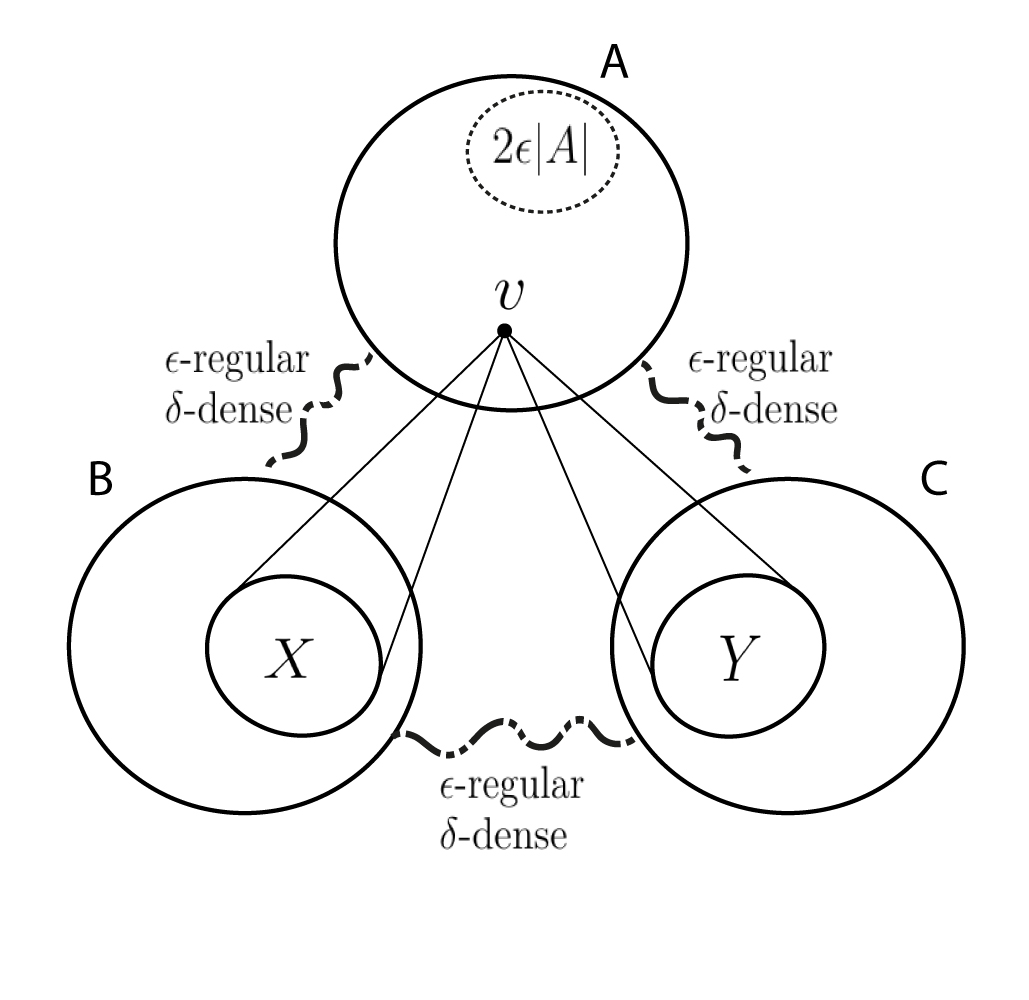
\includegraphics[scale=1]{Figuras/embedding-lemma.jpg}
     \caption{Triangles in the $\varepsilon$-regular pairs.}
     \label{fig:embeddinglemma}
\end{figure}

\end{proof}

\begin{theorem}[{The Szemerédi Regularity Lemma \cite{Sz75}}]. Let $\varepsilon > 0$, and let $m \in  \mathbb{N}$. There exists a constant $M=M(m,\varepsilon)$ such that the following holds.\\
For any graph $G$, there exists a partition $V(G) = \{V_0 \cup ... \cup V_k\}$ of the vertex set into $m \leq k \leq M$ parts, such that
\begin{itemize}

	\item $|V_1| = ... =|V_k|$,
	
	\item $|V_0| \leq \varepsilon|V(G)|$,
%$|A_0| \leq \varepsilon |V(G)|$,
	\item all but $\varepsilon k^2$ of the pairs $(V_i, V_j)$ are $\varepsilon$-regular. 
\end{itemize}
\end{theorem}

Note the lemma holds for all graphs, but it is useful only for graphs with large $n$ and with a minimum density.% Indeed, if $|V(G)| < M(m, \varepsilon)$ then each part has at most one vertex and if $e(G) = o(n^2)$ then $G$ is well-approximated by the empty graph, in both the lemma is vacuous and not so useful.  

\section{Applications}
Applying the regularity lemma, in general, has more convincing power of its use than the definitions or the proof of the lemma, then in this section we will show some classical applications. In order to apply the lemma we need to follow a standard process as can be seen below.

1. Apply the Szemerédi Regularity Lemma in order to acquire a partition $ \{ A_0, ... A_k \} $ as defined in the lemma.

2. Remove a few edges (edges inside the partitions, between irregular pairs and sparse pairs). There exist at most $O(\varepsilon n^2)$ such edges.

3. Define a graph $R$ such that $V(R) \rightarrow [k]$ and $\{i,j\} \in E(R) $ if  the pair $(A_i, A_j)$ is dense and $\varepsilon$-regular.

4. Apply a classical result from Graph Theory (e.g. Turán's Theorem) to R.

5. Apply the Embedding Lemma to find a copy of the desired subgraph $H$ in $G$.
\subsection{Erd\H{o}s-Stone Theorem}

\begin{theorem}[{Erd\H{o}s and Stone \cite{ErSt46}}] Let H be an arbitrary graph. Then
$$ \ex(n,H) = \left(1-\frac{1}{\chi (H)-1} + o(1)\right) \binom{n}{2}.$$ 
\end{theorem}

\begin{proof}


Assume $e(G) \geq (1 - 1/(\chi(H) - 1) + \delta)\binom{n}{2}$ and follow the steps above.

1. Apply regularity lemma with $\varepsilon$ sufficiently small and we have the partition $\{V_1, ... , V_k\}$.

2. Remove edges inside the parts, between irregular pairs and sparse pairs obtaining $G'$ as in Figure \ref{fig:graph-G-and-G'}.
Note that

|edges inside the parts| $\leq k\binom{n/k}{2} \leq k(n/k)^2 \leq \varepsilon n^2$ (recall $1/\varepsilon \leq k$).\\

|edges between not $\varepsilon$-regular pairs| $\leq \varepsilon k^2 (n/k)^2 = \varepsilon n^2$.\\

|edges between not $\delta$-dense pairs| $\leq \binom{k}{2}(\delta/4) (n/k)^2 \leq (\delta /4)n^2$.\\ 

Thus we have removed at most $(2\varepsilon + \delta/4)n^2$, therefore 

$$ e(G') \geq  \left( 1 - \frac{1}{\chi(H) - 1} + \frac{2 \delta}{3}\right) \binom{n}{2}.$$

\begin{figure}[H]
     \centering
     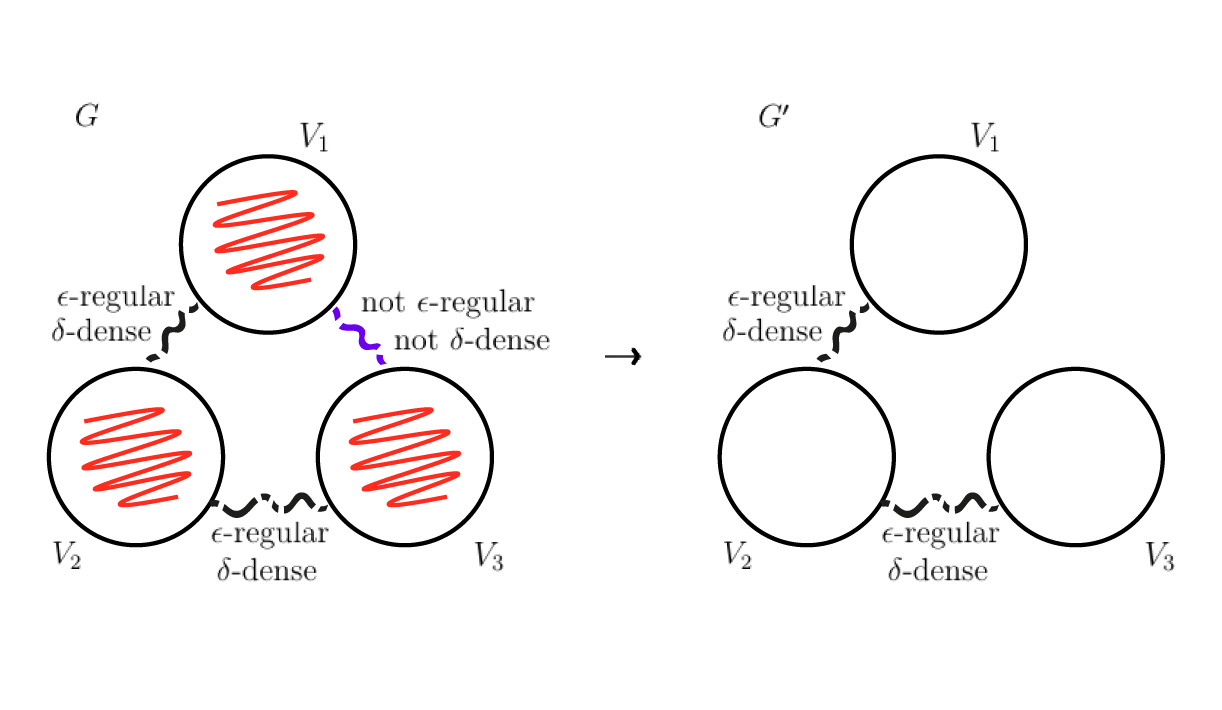
\includegraphics[scale=1.5]{Figuras/graph-G-and-G'.jpg}
     \caption{Graphs G and G'.}
     \label{fig:graph-G-and-G'}
\end{figure}

3. Define $R$ with $V(R) = [k]$ and $\{i,j\} \in E(R) $ if  the pair $(A_i, A_j)$ is dense and $\varepsilon$-regular as in Figure \ref{fig:graph-G'-and-R}

\begin{figure}[H]
     \centering
     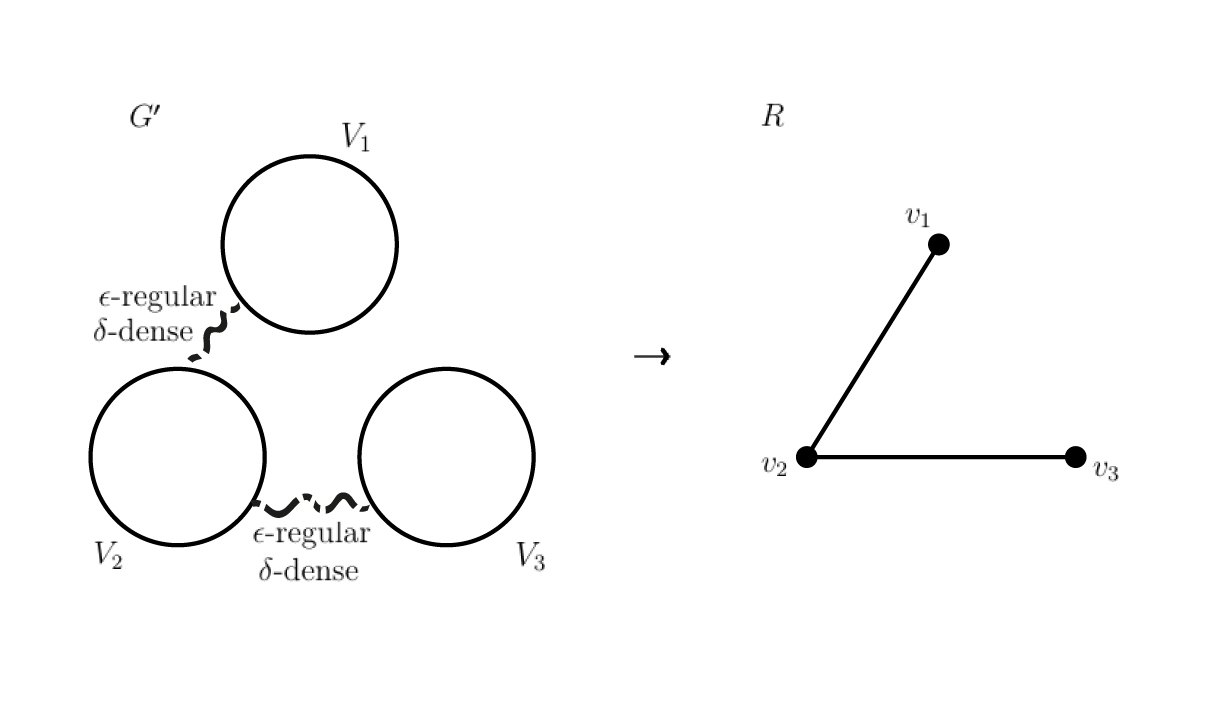
\includegraphics[scale=1.5]{Figuras/graph-G'-and-R.jpg}
     \caption{Graphs G' and R.}
     \label{fig:graph-G'-and-R}
\end{figure}

Note 
$$e(R) \geq \frac{e(G')}{\left(\frac{n}{k}\right)^2}.$$

4. Thus,
$$e(R) > \frac{\left(1 - \frac{1}{\chi(H) - 1} + \frac{\delta}{2}\right) \binom{n}{2}}{\left(\frac{n}{k}\right)^2} \approx \left( 1 - \frac{1}{\chi(H) - 1} + \frac{\delta}{2}\right) \binom{k}{2}> t_r(k),$$
we can apply the Turán's Theorem \ref{theorem:turan1941} that implies $K_{\chi (H)} \subseteq R$.

5. Now applying the Embedding Lemma \ref{lemma:embeddinglemma} with $n$ large enough follows that $H \subseteq G$ as required.

\end{proof}

\subsection{The Triangle Removal Lemma}
\begin{theorem}\label{lemma:triangleremoval}[{Triangle Removal Lemma \cite{RuSz76}}]
For all $\alpha > 0$ exists $\beta > 0$ such that if $G$ is a graph with $\leq \beta n^3$ triangles, then it is possible to remove all triangles removing at most $\alpha n^2$ edges. 
\end{theorem}

\begin{proof}
The first, second and third steps of the method are, in general, the same for classical problems,

1. Apply SzRL with $\varepsilon$ enough small and we have the partitions $\{V_1, ... , V_k\}$.

2. Remove edges inside the partitions, between irregular pairs and sparse pairs obtaining $G'$ with at most $\alpha n^2$ edges removed.

3. Define $R$ with $V(R) = [k]$ and $\{i,j\} \in E(R) $ if  the pair $(A_i, A_j)$ is dense and $\varepsilon$-regular.

Now we have two cases, in the first one we have a triangle in $R$. Note if $\beta n^3 < 1$ the result is trivial, then we assume $\beta \geq 1/n^3$ and the partitions that forms the triangle (assume $\{V_1, V_2, V_3\}$ for simplicity) has size $n/k \geq 1/(\beta ^{1/3} k) \geq m$.

Applying the Embedding Lemma \ref{lemma:embeddinglemma} we have that the quantity of triangles in $G'$ is at least $\delta ^3 /2 (n/k)^3 > \beta n^3$ if we choose $\beta$ such that $\delta ^3 / (2k^3) > \beta$.

We conclude that if $\alpha n^2$ edges are removed and the graph still has triangles the triangles quantity is more than $\beta n^3$.

In the second case there is no triangle in $R$ and this implies there is no triangle in $G'$ because the edges inside the pairs $\{V_1, ... , V_k\}$ were removed then the only possible triangles are formed between the pairs, finishing the proof.
\end{proof}


\subsection{Roth's Theorem}

\begin{theorem}[{Roth's Theorem \cite{Ro53}}] If $A \subseteq \mathbb{N}$ has positive upper density, then $A$ contains an arithmetic progression of length three. 
\end{theorem}

\begin{proof}
Choose $\delta > 0$ with $|A \cap [n]| > \delta n$, with $n$ sufficiently large. Let $V(G) = X\cup Y \cup Z$, where $X, Y$ and $Z$ are disjoint and $X,Y,Z \subseteq [n]$ and let,

\begin{align*}
E(G) &= \{\{x,y\}\colon x \in X, y \in Y,\text{ and } y = x + a, a \in A\} \\
& \cup \{\{y,z\} \colon y \in Y, z \in Z, \text{ and } z = y + b, b \in A\}\\
& \cup \{\{x,z\} \colon x \in X, z \in Z, \text{ and } z = x +2c, c\in A\}
\end{align*}

Note if $A$ has no $3$-AP, then all the triangles in $G$ correspond to triples $\{a,a,a\}$ and there exist $n|A\cup [n]| \leq n^2$ such triangles. Suppose we have no $3$-AP in A.
 
 Then we can apply the Triangle Removal Lemma \ref{lemma:triangleremoval} to $G$ for n sufficiently large, which means we can destroy all triangles in $G$ by removing at most $\alpha n^2$ edges. But these triangle triples $\{a,a,a\}$ are edge-disjoint and we have more than $\alpha n^2 $ such triangles which is a contradiction, finishing the proof.
 
\end{proof}

\chapter{Conclusion}
Essential classical results and methods in Extremal Combinatorics were presented in this project, although it is not a complete cover of literature it gives us a good background of this fruitful area of study and makes easier to expand knowledge and results throughout the whole area of Extremal Combinatorics. We focus our efforts in the methods and results we consider most important and useful for who is interested in continuing studying the area in postgraduate courses and contributing for the area expansion in the future.

We use as base text and initial point of study the Robert Morris and Roberto Imbuziero book \cite{RoRo11} which cover more topics of study and is much more simplified and	 summarized. Completing the gaps and trying to make a self-contained text with detailed explanations for initial students of the area was a great effort by itself.




%BIBLIOGRAFIA
\bibliographystyle{amsplain}
\bibliography{minhabib}

\end{document}

%%% Local Variables:
%%% mode: latex
%%% eval: (auto-fill-mode t)
%%% eval: (LaTeX-math-mode t)
%%% eval: (flyspell-mode t)
%%% TeX-master: t
%%% En